\documentclass{sig-alternate}
\usepackage{subfigure}
\usepackage{url}
\usepackage{multirow}
%\usepackage{wrapfig}
\usepackage[ruled,vlined]{algorithm2e}
%\usepackage{algorithm}
%\usepackage{algorithmic}
\newdef{definition}{Definition}
\newdef{example}{Example}
%\newdef{balabala}{Rule}
%\newtheorem{algorithm}{Algorithm}

\usepackage[usenames]{color}
\newcommand{\comment}[1]{{\color{Magenta}{#1}}}

\begin{document}
%
% --- Author Metadata here ---
\conferenceinfo{CIKM}{'13 San Francisco, CA USA}
%\CopyrightYear{2007} % Allows default copyright year (20XX) to be over-ridden - IF NEED BE.
%\crdata{0-12345-67-8/90/01}  % Allows default copyright data (0-89791-88-6/97/05) to be over-ridden - IF NEED BE.
% --- End of Author Metadata ---

\title{Matching Millions of Queries with Billions of Bid Keywords}
%\titlenote{(Produces the permission block, and
%copyright information). For use with
%SIG-ALTERNATE.CLS. Supported by ACM.}}
%\subtitle{[Extended Abstract]
%\titlenote{A full version of this paper is available as
%\textit{Author's Guide to Preparing ACM SIG Proceedings Using
%\LaTeX$2_\epsilon$\ and BibTeX} at
%\texttt{www.acm.org/eaddress.htm}}}

%\numberofauthors{8} %  in this sample file, there are a *total*
%\author{
% 1st. author
%\alignauthor
%Ben Trovato\titlenote{Dr.~Trovato insisted his name be first.}\\
%       \affaddr{Institute for Clarity in Documentation}\\
%       \affaddr{1932 Wallamaloo Lane}\\
%       \affaddr{Wallamaloo, New Zealand}\\
%       \email{trovato@corporation.com}
% 2nd. author
%\alignauthor
%G.K.M. Tobin\titlenote{The secretary disavows
%any knowledge of this author's actions.}\\
%       \affaddr{Institute for Clarity in Documentation}\\
%       \affaddr{P.O. Box 1212}\\
%       \affaddr{Dublin, Ohio 43017-6221}\\
%       \email{webmaster@marysville-ohio.com}
% 3rd. author
%\alignauthor Lars Th{\o}rv{\"a}ld\titlenote{This author is the
%one who did all the really hard work.}\\
%       \affaddr{The Th{\o}rv{\"a}ld Group}\\
%       \affaddr{1 Th{\o}rv{\"a}ld Circle}\\
%       \affaddr{Hekla, Iceland}\\
%       \email{larst@affiliation.org}
%\and  % use '\and' if you need 'another row' of author names
% 4th. author
%\alignauthor Lawrence P. Leipuner\\
%       \affaddr{Brookhaven Laboratories}\\
%       \affaddr{Brookhaven National Lab}\\
%       \affaddr{P.O. Box 5000}\\
%       \email{lleipuner@researchlabs.org}
% 5th. author
%\alignauthor Sean Fogarty\\
%       \affaddr{NASA Ames Research Center}\\
%       \affaddr{Moffett Field}\\
%       \affaddr{California 94035}\\
%       \email{fogartys@amesres.org}
% 6th. author
%\alignauthor Charles Palmer\\
%       \affaddr{Palmer Research Laboratories}\\
%       \affaddr{8600 Datapoint Drive}\\
%       \affaddr{San Antonio, Texas 78229}\\
%       \email{cpalmer@prl.com}
%}
% There's nothing stopping you putting the seventh, eighth, etc.
% author on the opening page (as the 'third row') but we ask,
% for aesthetic reasons that you place these 'additional authors'
% in the \additional authors block, viz.
%
%\date{30 July 1999}
%
% Just remember to make sure that the TOTAL number of authors
% is the number that will appear on the first page PLUS the
% number that will appear in the \additionalauthors section.

\maketitle
\begin{abstract}
  Sponsored search is the main source of revenue of a search engine.
  Advertisers bid on phrases for their advertisements, and search
  engines match user queries to relevant ads based on the bid phrases.
  Since both queries and bid phrases are short texts and cannot be
  modeled by the standard bag-of-words approach, most existing
  approaches exploit user behavior data (e.g., click-through data,
  session data, etc.) to fill the semantic gap in matching bid phrases
  and user queries. This approach however cannot handle tail queries
  which do not have much user behavior data.  Although individually
  rare, tail queries as a whole account for a considerable portion of
  the query volume and are a significant source of search engine's
  revenue.  In this paper, we propose a novel approach for matching
  queries and bid phrases.  Leveraging a probabilistic taxonomy and a
  large scale term co-occurrence network, we conceptualize a short
  text to a set of relevant concepts.  To handle millions of queries
  and billions of bid phrases, we create a semantic index of
  concepts: relevant bid phrases are selected for a given query by
  measuring their similarity in the concept space.  We conduct a
  series of experiments including expanding 30 million queries with
  0.7 billion phrases.  Experiment results show the effectiveness of
  our approach.
\end{abstract}

% A category with the (minimum) three required fields
\category{H.3.3}{Information Storage and Retrieval}{Information Search
and Retrieval}
%A category including the fourth, optional field follows...
%\category{D.2.8}{Software Engineering}{Metrics}[complexity measures, performance measures]

\terms{Algorithm, Experimentation}

\keywords{Sponsored advertising, query expansion, keyword suggestion,
    text modeling}

%Basically, our story is this:
%
%In sponsored search, we need to find matching bid keywords for a
%query.
%
%Semantic problem: matching must be semantic, but both keywords and
%query are short texts.
%
%Scalability problem: there are billions of bid keywords.
%
\section{introduction}
%What's sponsored search
Sponsored search aims at matching search queries to relevant
advertisements.  Each ad is characterized by a list of bid keywords
which are representative for it.  If the matching option is
\emph{exact match}, an ad has opportunity to be triggered if the given
query is identical to one of its bid keyword.  Another option is
\emph{smart match} which is the default option provided by mainstream
search engines.  In this scenario, search engines display ads whose
bid keywords are semantically relevant to the given query.  Smart
match can potentially channel a larger traffic volume to
advertisers~\cite{wang:advertisementsearch}. However, in most cases,
    this traffic is less targeted compared with exact match.  Our
    paper deals with finding matching bid keywords for a qeury and
    focus on the semantic relevance between sthem.


%Semantic problem
Both queries and bid keywords are very short (the average length is
        between 2.4 and 2.7 words~\cite{broder:webknowledge}).  Thus
matching based on syntactic similarity suffers from low
recall~\cite{wang:advertisementsearch}.  As a result, only 30\%-40\%
of search queries are covered by ad
results~\cite{broder:sponsoredsearch}.  To address such serious word
mismatching problem, matching must be semantic.  Topic
models~\cite{blei:dirichletallocation, deerwester:semanticanalysis}
express semantics as distribution over latent topics.  They are useful
for corpus of normal documents, but queries as well as bid keywords are too short to
provide statistically meaningful signals.  A more promising approach
is to augment queries with additional external 
knowledge such as user behavior data~\cite{cui:querylogs,
    broder:webknowledge, fuxman:keywordgeneration}.  However, they are
    only effective for popular queries, but not for \emph{tail
        queries} that have little or no historical user behavior data.
        Unfortunately, tail queries, though individually rare, make up
        a significant portion of the query
        volume~\cite{broder:sponsoredsearch}.


No matter a query is popular or rare, human beings can understand it
easily.  This is because knowledge in a human mind makes up for the
sparsity of the input.  If we can provide such knowledge to machines
         then they can better understand short texts.  Gabrilovich et
         al~\cite{gabrilovich:semanticanalysis} proposed a novel
         approach known as {\em explicit semantic analysis (ESA)},
         which models a short text by a set of
         Wikipedia~\cite{wiki:tool} concepts (it considers the title
                 of any Wikipedia article as a Wikipedia concept).
         However, such taxonomy-based approach relies on the quality
         and coverage of the taxonomy~\cite{chen:concepthierarchy} and
the concept space of Wikipedia is limited (about 111,654
        concepts~\cite{wu:manyconcepts}).
Besides, the transformation from bag-of-words to bag-of-concepts in
ESA is based on co-occurrence between terms of a short text and terms
in Wikipedia articles.  However, most terms in an article do not have
\emph{isA} relationships with the corresponding Wikipedia concept.
Therefore, associating short texts with their relevant concepts via
this co-occurrence information is not precise.  We regard the
co-occurrence information used for \emph{conceptualization} in their
approach as \emph{loose isA} relationship.  For a short text, its limited
number of terms makes the loose isA relationship more vulnerable.


In our approach, we expand a sparse, noisy and ambiguous input to a
rich, explicit, and accurate representation via \emph{strict isA}
relationships provided by probabilistic taxonomies such as
Probase~\cite{wu:manyconcepts} and Yago~\cite{SuchanekKW07yago}.  Then
we perform similarity calculation on that representation. Our
conceptualization algorithm associates each short text with
its relevant concepts by inferencing technique based on probabilities
provided by adopted taxonomy.  We also mine frequent sense-patterns
from the adopted co-occurrence network and filter inappropriate
concepts assigned to short texts to avoid additional noise. 


%scalability problem
Besides of semantic problem, scalability is critical for any sponsored
search approaches. Moreover, in our approach, each short text is
mapped into concept space and has a distributed representation.
Thus matching between short texts over our enriched representation is
more complicated compared with the matching between bags-of-words
(around 2 words).  Comparing millions of queries with billions of
keywords by a naive algorithm is intractable even in our map-reduce
cluster. Thus, instead of assigning a score to each bid keyword
and ranking the entire corpus, we leverage locality-sensitive hashing
(LSH) to efficiently select a small set of relevant bid keywords
before ranking.


In summary, we make the following major contributions:
\begin{itemize}
\item We propose a new approach for query expansion.  Our approach is
much more \emph{robust} because: (1) We leverage web-scale,
     data-driven knowledgebases, and (2) we conceptualize short texts
     through strict isA relationships which are more reliable than
     through loose isA relationships.
\item We propose a sophisticated algorithm to conceptualize short
  texts.  Our algorithm resolves word mismatching problem by
  ``lifting'' the representation of short text to the concept level.
  Besides, it mines frequent sense-patterns to eliminate ambiguity of
  short text.
\item Our approach can match both head and tail queries to relevant
  bid keywords.  This is very critical for current sponsored search
  systems since selecting relevant ads for tail queries is the major
  bottleneck.
\item Our approach can scale to massive datasets.  
%Instead of
  %assigning a score to each bid phrase and ranking the entire corpus,
  %we leverage locality-sensitive hashing (LSH) to efficiently select a
  %small set of relevant bid phrases before ranking.  
  We apply our
  approach to expand 30 million queries with 0.7 billion bid keywords
  for a commercial search engine.
\end{itemize}


The rest of this paper is organized as follows.  In the next section,
    we summarize related work.  We introduce the external resources
(knowledgebases) used in our approach in Section 3.  In Section 4, we
give a brief introduction to our system architecture.  We present our
conceptualization algorithm in Section 5.  In Section 6, we describe
the process of selecting and ranking candidates to derive final
results.  Experiments are discussed in Section 7.  We conclude our
paper in Section 8.

\section{Related Work}
Techniques proposed in this paper are related to keyword suggestion
and query expansion.



Because the average length of queries are around
2~\cite{baeza:searchengines}, query expansion has been thought as an
effective way to resolve word mismatching
problems~\cite{cui:querylogs}.
Existing approaches mainly focus on expanding queries with various
external resources including organic search
results~\cite{broder:relevancefeedback, joshi:engineadvertising}, user
behavior
data~\cite{cui:querylogs,broder:webknowledge,fuxman:keywordgeneration}
and bidding relationships between phrases and
ads~\cite{wang:advertisementsearch}.
%Modern search engines can return decent organic search
%results even the search query is very short.
%Fertilizing queries with algorithmic search results would bring in
%unacceptable latency for sponsored advertising and can't be applied
%real-time.
%User behavior data including click-through data, query session data
%may capture the semantic relevance between search phrases.
Ricardo et al~\cite{baeza:searchengines} propose to represent queries
by aggregation of terms-weight vectors of their clicked URLs, which
leverages both organic search results and user behavior data.
However, in most cases, there is no adequate user behavior data for
tail queries that are individually rare but make up a significant
portion of the query volume~\cite{broder:sponsoredsearch}.



%Text snippets are firstly mapped into their concept hierarchy.
%Then the similarity between original text snippets are measured by
%similarity between their corresponding set of concepts using
%conventional metrics.
%To fill the gap between the keywords chosen by advertisers and their
%potential customers, keyword suggestion technology is employed.
%Chen\cite{chen:concepthierarchy} exploits the semantic knowledge
%derived from open directory project(ODP)\cite{odp:tool}.
%Query is firstly mapped into their concept hierarchy.
%Then the new keywords are suggested according to the concept
%information of original keyword.
%As they pointed, their approach is directly affected by the quality
%and the coverage of the concept hierarchy.
%However, they consider categories in ODP as the concepts in their
%hierarchy and unfortunately there are only about 150,446 ODP
%categories.
%Cao\cite{cao:sessiondata} propose clustering queries based on
%click-through data and making context-aware suggestion by mining
%session data.\\
%For search engines, the most important task for them is to match
%users' submitted queries to relevant ads.
%Traditionally, sponsored search employed standard information
%retrieval techniques using the bag of words(BoW) approach.
%Since BoW model ignores relations between words and can not access the
%semantics behind text.
%It is challenging to identify relevant ads for user's query when the
%query is very short.
%In fact, web users usually issue very short queries to search engines
%whose average length is less than two words\cite{wen:searchengine}.
%Besides, users typically choose terms intended to achieve optimal web
%search results rather than optimal ads and ads themselves are also
%very short in most cases\cite{broder:relevancefeedback}.
%Classical works related to such task employed various resources as
%additional knowledge to enrich the features of short queries.
%Using organic search results to provide greater context for the short
%texts are widely accepted\cite{broder:relevancefeedback}.
%User behavior data including click-through data, user query session
%and bidding information are used to derive information about
%similarity between terms or short texts.
%Cui\cite{cui:querylogs} exploits correlations among terms in documents
%and user queries mined from user logs.
%Wang\cite{wang:advertisementsearch} propose clustering queries based
%on the bipartite graph between queries and ads.
%Approaches making full use of taxonomy work in explicit semantic
%analysis(ESA)\cite{gabrilovich:semanticanalysis} manner.
%There are various taxonomies are used for query expansion including
%Wikipedia\cite{hu:withwikipedia}, open directory
%project(ODP)\cite{chen:concepthierarchy} and
%WordNet\cite{voorhees:semanticrelations}.
%Some techniques combining various additional resources to be used are
%proposed.
%Broder\cite{broder:sponsoredsearch} enrichs the features of head
%queries with organic search results offline and online expands rare
%queries by retrieve related head queries from a vector space model
%using textual features as well as semantic-class features.
%Query expansion research has more than three decades history and we
%can't introduce all the classical works here.
%\cite{carpineto:informationretrieval} is a detailed and genealogical
%survey on query expansion.\\
More fundamentally, the key problem of many queries processing tasks
and keyword research is measuring similarity between short texts.
Previous work on measuring text semantic similarity has focused mainly on either large
documents or individual words~\cite{mihalcea:semanticsimilarity}.
Since both queries and bid phrases are too short to draw reliable
statistical conclusion, LSA approaches~\cite{blei:dirichletallocation,
    deerwester:semanticanalysis, hofmann:semanticindexing} are not an
    effective way to index short text snippets.
Besides corpus-based approaches, existing approaches for measuring
short text semantic similarity are largely
knowledge-based~\cite{gabrilovich:semanticanalysis,hu:withwikipedia,chen:concepthierarchy,song:probabilisticknowledgebase}.
Knowledgebase including WordNet~\cite{wordnet:tool}, open directory
project(ODP)~\cite{odp:tool} and wikipedia\cite{wiki:tool} are
exploited to enrich short text snippets at semantic level.
As Chen et al~\cite{chen:concepthierarchy} pointed, the performance of
knowledge-based approaches are strikingly affected by the accuracy and the coverage
of used concept hierarchy.
%and unfortunately there are only about
%150446 ODP categories which are considered as concepts in their
%approach.
Our approach model and rank short text with the help of a probabilistic taxonomy
named Probase~\cite{wu:manyconcepts} which, to the best of our
knowledge, contains the largest concept space compared with those
knowledgebases adopted by existing approaches.
Besides, most of these knowledge-based approaches map short text
snippets into their concept space based on co-occurrence of terms
within the content of original text and terms appearing in
corresponding articles or web pages of concepts.
Considering that queries and bid phrases are very short, such strategy
is not reasonable.

\section{The Knowledgebase}
\label{sec:knowledge}
The emergence of large scale, probabilistic knowledgebases, such as
Probase~\cite{wu:manyconcepts} and Yago~\cite{SuchanekKW07yago},
brings new opportunities to text understanding.  We adopt Probase, a
probabilistic taxonomy for conceptualization in our approach.  The
reason we prefer Probase is that we consider a huge concept space
indispensable to understand open-domain bid phrases. Probase is rich
enough to cover a large proportion of concepts about worldly facts.
The version of Probase we use contains about 8.26 million instances
(e.g., ``windows phone 7'', ``ipad'', ``kindle'', etc.) and about 2.7
million concepts (e.g., ``platform'', ``device'', ``ebook reader'',
etc.).  In the rest of this paper, we use $e$ to denote an instance, $c$
as a concept.

All instances and concepts are organized hierarchically by the
\emph{isA} relationships.  For example, ``kindle'' is an instance of
concept ``ebook reader''.  Note that \emph{isA} relationships also
exist between sub-concepts and concepts (e.g., sub-concept ``ebook
reader'' is an instance of concept ``device'').  In contrast to
traditional taxonomies that regard knowledge as black and white,
Probase maintains probabilistic \emph{isA} relationships:
\begin{eqnarray}
%\begin{aligned}[b]
\Pr(e\vert c)=\frac{n(e,c)}{n(c)}\>\>\>\>\>\> \Pr(c\vert e)=\frac{n(e,c)}{n(e)}
%\Pr(c\vert e)=\frac{n(e,c)}{n(e)}
%\end{aligned}
\end{eqnarray}
where $n(c)$, $n(e)$, $n(e,c)$ denote the frequency of $c$, the
frequency of $e$, the frequency of $e$ and $c$ occuring together in all
Hearst patterns~\cite{Hearst92} extracted from billions of documents
and web pages.  These probabilities have some natural properties:
$P(e\vert c)$ reflects the typicality of $e$ given
$c$, and $P(c\vert e)$ reflects the typicality of
$c$ given $e$.  We use these probabilities as fundamental building blocks
for probabilistic models to conceptualize short texts.



We also use Probase's instance-instance co-occurrence network wherein each
node is a Probase instance and each edge between two nodes is the
co-occurrence relationship between instances.  For 8.26 million
instances, we extract their co-occurrence relationships from 1.68
billions of web pages.  Each time two instances co-occur within one
sentence of those web pages, we will increase their co-occurrence
frequency by 1.  Finally, we got a weighted network with 28.6 billion
edges.  After some filtering (such as removing edges with frequency
$\leq 5$), the ultimate network contains about 3.73 billions of edges.
We will use this co-occurrence information to disambiguate multiple
concepts of an instance to avoid enriching instances with noisy concepts.
%
%
%
%Clicks define a strong associations between queries and URLs.
%The semantics of a query is captured by its clicked
%URLs~\cite{fuxman:keywordgeneration}.
%Since our setting is sponsored search, we also exploit such valuable
%external knowledge.
%Our click-through data is collected through a commercial search engine
%and a mainstream web brower during one month period.
%Although the click-trhough data records various information, we are
%only interested in clicked URLs and search phrases.
%Thus, in the rest of this paper, we denote click-through data as tuples $Click Data=\{(q,u)\vert
%q\in Q,u\in U\}$ where $Q$ denotes all the search phrases and $U$
%denotes all the URLs.
%There are around 1.5 billions of such kind of tuples in our
%click-through data.


%%% Local Variables:
%%% mode: latex
%%% TeX-master: "adselection"
%%% End:

\section{System Framework}
In this section, we present the system diagram (Figure
\ref{fig:framework}), which shows how data flows through our system
end-to-end.  Just like classical IR systems, it can be divided into
online and offline components.

\begin{figure}[!htbp]
\centering
%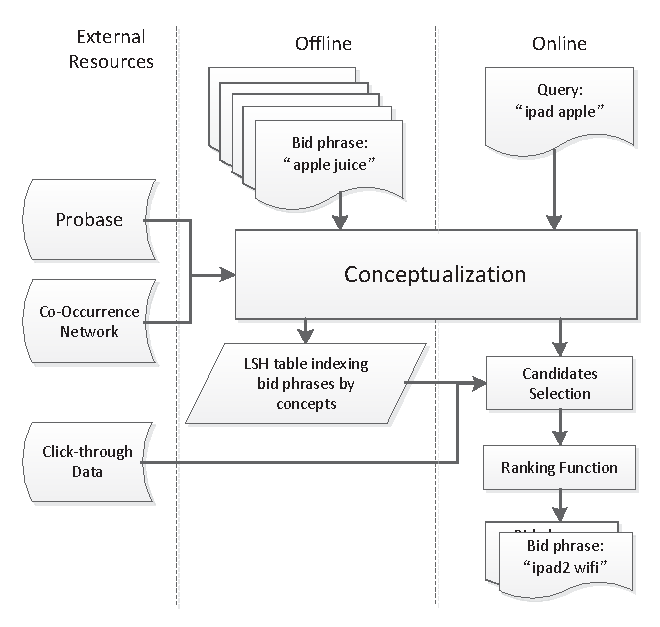
\epsfig{file=figures/frameworkv2.eps, width=3.3in}
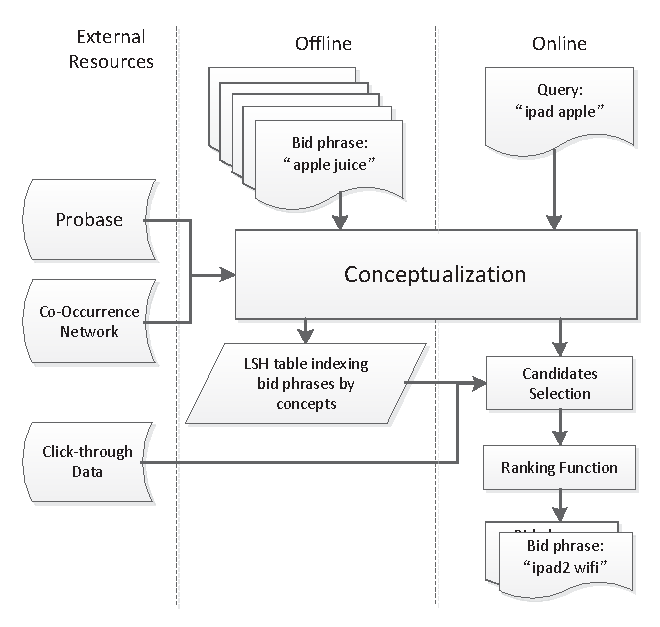
\includegraphics[width=3.3in]{figures/frameworkv2.eps}
\caption{Overall System Architecture}
\label{fig:framework}
\end{figure}
%We also include a module in our framework that evaluate and tune the
%resulting suggestions(expansions) based on statistics collected from
%actual combat.



In offline processing, we conceptualize each bid phrase, that is, we
map each bid phrase to a set of representative concepts.  This enables
us to estimate the similarity between two short texts by measuring the
similarity between their corresponding sets of concepts.  For the
purpose of large scale similarity computation, we exploit the
locality-sensitive hash (LSH) scheme to index bid phrases.  LSH
enables us to efficiently find bid phrases whose corresponding concept
sets are likely to be similar to that of the query.  Besides, we also
mine click-through data to extract semantic associations (i.e.,
co-click relationships) between queries and index them for efficient
real-time looking up.  At runtime, when a query is posed, we
conceptualize it in the same way as we did for bid phrases.
%Because the number of bid phrases contained by search engine is
%extremely large, comparing a given query with each bid phrase on
%their rich conceptualization results can't satisfy efficiency
%requirements of online system.
%Because the number of bid phrases is usually in the order of
%billions, it is not feasible to compare the concept representation of
%the query with that of each bid phrase.  In order to make our approach
%efficient enough to handle the massive amount of bid phases, we
Then, from the massive bid phrase dataset, we select a small
set of bid phrases that are relevant to the given query using 
user behavior data (for head queries) or 
%and 
LSH (for tail queries).
%portion from the entire corpus of
%bid phrases as candidates that are somewhat relevant to the given query.%for further consideration.
Finally, we rank these candidates and use the top-ranking ones as
query suggestions (expansions).
%If the given query has enough
%For queries that have sufficient click-trhough data to draw reliable
%conclusion on which bid phrases are relevant to it, we select bid
%phrases as candidates for it based on such information.
% If the query is a term of our pre-built index that contains co-click
% relationships, we simply select bid phrases from the posting list of
% the term as candidates.
% Otherwise, we look the conceptualization result
% of the given query up in the LSH tables and use retrieved bid phrases as
% candidates.
%Finally, we apply our ranking function to re-order
%selected candidates and reserve the top ranking ones as final results.



%Such task should be finished efficiently while ensuring the quality of
%candidates.
%We design two approaches for candidates selection.
%One approach leverage semantic associations provided by click-through
%data by looking up our lookup table to select associated search phrases.
%So our another approach only focus on conceptualization results.
%we look the conceptualization result of given query up in
%the LSH table and use those retrieved bid phrases as candidates.
%As an efficient real-time system, we can apply our approach to
%preprocess a large collection of queries without any additional
%difficulty.
%The resulting lists of bid keywords can be used as suggested keywords
%or query's expansions for sponsored search.
%Actually, we use a small portion of search engine's traffic volume to
%evaluate our results.
%According to collected statistics, we tune the setting of our approach
%improve better suggestions(expansions).
%\comment{{do we need to claim we get good resutls in the flight?}}


%%% Local Variables:
%%% mode: latex
%%% TeX-master: "adselection"
%%% End:

\section{Conceptualization}
Conceptualization generalizes input to concepts. It is one of the most
basic cognitive process for human beings.  For instance, we generalize
``hot dog'' to the concept of ``food'', and ``dog'' to the concept of
``animal''.
%To do this, we need knowledge.  Probase provides rich
%conceptual knowledge that covers most worldly concepts, and allows
%machines to handle text understanding tasks as humans do.
To allow machines to handle such text understanding tasks, we exploit
rich conceptual knowledge provided by Probase that covers most worldly
facts.
%We divide the process of conceptualizing short text into three phases:
%(1)identifying entities from the short text;
%(2)inferring topics based on observed entities;
%(3)word sense disambiguation(WSD) by mining frequent
%concept-patterns.
\subsection{Instances Detection}
%By tokenization, each short text is regared as a sequence of tokens
%$T=\{t_i,i\in1,\ldots,L\}$.
%Say that an entity $e$ covers $T[i,j](j\geq i)$ if the consecutive
%subsequence of $T$ from $t_i$ to $t_j$ is identical to $e$.
%We detect entities from content of short text according to the
%following rule:
%\begin{balabala}
%$\forall i\in 1,\ldots,L$,identify $e$ which covers $T[i,j](j\geq
%        i)$ s.t. $\forall e^{'}$ that covers
%$T[i^{'},j^{'}](j^{'}\geq i^{'}),i^{'}\leq i\to j^{'}<j$
%\end{balabala}
%We consider each position in the token list as beginning position of
%eneity expecting to extract as many appropriate entities as possible
%so that they may provide richer hints of the semantics behind observed
%short text.
Given a short text such as ``windows phone app'', %we detect instances within the short text using a
%naive approach.
We firstly identify all Probase instances that appear
in the short text---``windows'', ``windows phone'', ``phone app'' and
``app''.  Next, we remove an instance if it is entirely
covered by another one (that is, it is a substring of another
instance). Thus after this step, our example short text is transformed
into a set of Probase instances $\{\text{``windows
    phone''},\text{``phone app''}\}$. 
%The reason we prefer instances of longest lengths lies in the
%fact % that compond words of open
% form % \footnote{there is space between
%   % each word of which the compound one consists} 
% are ubiquitous in
% English.  
%in most cases, the meaning of a compound word is a specialization of
%the head word.  In other words, 
In fact, an instance entirely covered by another
instance is very likely to be either its modifier or its head that has a
more general meaning.  Because conceptualization ``lifts'' the
representation of short text from term-level to concept-level, more
specific instances are better for avoiding ``over-abstracting''.%semantic drift.
%For
%example, within the short text ``windows phone app'', there are
%Probase instances $\textnormal{``windows''}_1$, $\textnormal{``windows
%  phone''}_1$, $\textnormal{``phone app''}_2$ and
%$\textnormal{``app''}_3$.  Note the subscript index indicates the
%beginning position of each instance.  We select ``windows phone''
%instead of ``windows'' becuase it is the longest cover beginging at
%position $1$.  Since ``app'' is entirely included by ``phone app'', we
%filter it even though it is the longest cover of position $3$.
%\end{example}
\subsection{Senses Derivation}
%The second step is to derive senses from observed entities.
%In our approach, each sense is characterized by a cluster of related
%concepts.
%In Probase, each entity is associated with a number of concepts that
%are the hypernyms of this entity.
%However, there are considerable number of ambiguous entities whose
%concepts should be partitioned into several clusters where each
%cluster expresses one sense of it.
%In Probase, Each instance $e$ maps to a set of concepts
%$\{c\vert\Pr(c\vert e)>0\}$. For each instance, we use an offline
%process to cluster its concepts and each cluster of concepts is
%treated as one sense of the instance.
%For example, the term ``apple'' may associate with one cluster
%that contains concepts such as ``fruit'', ``juice'', and another
%cluster that contains concepts such as ``company'', ``brand'', etc.
Sense of a word or phrase is its meaning.  To represent one sense of
an instance, we use a set of related concepts.  
See Table \ref{tab:re} for example, the set of all ``ipad'''s concepts $\{c\vert\Pr(c\vert
        \text{``ipad''})>0\}$ represents its only sense.
However, ambiguous instances such as ``apple'' has more than one sense and
associates totally unrelated concepts (e.g., ``fruit'' and ``company'')
in Probase.  We use an offline process to partition each instance's
concepts into one or more clusters where each cluster consists of
related concepts and thus represents one sense of the instance.
%Firstly, for each detected entity, we rank concepts of Probase by
%their likelihood given the entity(i.e., $\Pr(c\vert e)$) and reserve
%the top-$K$ concepts.
%Thus, each observed entity is associated with a concept vector
%$\mathbf{c}=(c_1,c_2,\ldots,c_{\vert C\vert})$.
%Note that normalization is needed because reserving only top-$K$
%concepts means truncating the entity's original distribution over
%concepts.
%Because number $K$ is usually of tens order, the concept vector
%$\mathbf{c}$ is extremely sparse compared with the dimensionality of Probase's concept space.
%However, transforming a short text containing only two or three terms
%into tens of explicit concepts is really an enrichment.
%Secondly, we split concept vectors of ambiguous entities.
%Actually, we cluster concepts within a concept vector $\mathbf{c}$
%based on the \textit{isA} relationships within them and the similarity
%between their entities as shown in Algorithm \ref{alg:clustering}:
% For clustering, how to decide initial clusters and how to determine
% the number of clusters are critical problems.  


%We devise a clustering algorithm (see Algorithm~\ref{alg:clustering})
For each instance $e$, we cluster its associated concepts by exploiting
\emph{isA} relationships and typicality.
% The most typical concepts of an entity
% are general, popular and thus representative for
% senses(clusters).%to which they belong.
% %Besides, the \emph{isA} relationships provided by Probase are of high quality
% %and more reliable than any statistical information.
% Our concept clustring algorithm is 
Given an instance $e$, we first rank its concepts by typicality (i.e.,
$\Pr(c\vert e)$) and select the top-$K$ most typical concepts for $e$.
The value of $K$ is usually in the order of tens (in our
        implementation $K=15$).  Then, we cluster the $K$ concepts
agglomeratively.  At the beginning, each of the $K$ concepts is
regarded as an independent cluster.  During the procedure, if there
exists isA relationship between any two concepts, their clusters are
merged.


Indeed, mainstream taxonomies (either automatically generated or
        manually annotated) are rather clean but not complete enough. 
For example, there is no isA relationship between the concept
``conventional input device'' and any other concepts in the first
sense (cluster) of ''mouse'' (see Table \ref{tab:iniclusters}).
%and thus it can't
%be absorbed into the first cluster of ``mouse'' due to the imcomplete
%isA relationships of Probase.
However, we can eventually merge them correctly by a simple rule: if a
certain concept is the suffix of another concept, merge their clusters
together. Actually, ``device'' is the head of not only ``conventional
input device'' but also most concepts in the first sense of ``mouse''.
%identify its correct sense
%by the fact that it share a common 
%One suffix of ``conventional input device'' is ``device'' and with many
%concepts of that sense and ``device'' itself is actually the head of
%most concepts of that sense.
%Up to now, if a concept still forms a cluster alone, we merge it with the cluster
%whose concepts has the largest number of intersecting hypernyms with it among
%all the clusters.
%\\in reality, I add the above heuristic rule for concept clustering,
    %however, we'd better eliminate it in our paper.


This procedure results in several initial clusters. Table
\ref{tab:iniclusters} shows initial clusters of some ambiguous
instances.  Let the instances of a cluster be the union of its
concepts' instances, we can assign other concepts associated with $e$
%(i.e.,
%$\{c\in C\vert\Pr(c\vert e)>0\}$) 
    to its closest cluster where
``closeness'' is measured by the proportion of overlapping instances
of them. % is represented by its
% distribution over all Probase's entities and each cluster is
% reresented by the mean of its initial concepts' representations.
% Cosine distance is adopted for distance measurement.
%\IncMargin{1em}
%\begin{algorithm}[!tb]
%\SetKwInOut{Input}{input}
%\SetKwInOut{Output}{output}
%\caption{CONCEPT CLUSTERING}
%\Input{instance $e$ and parameter $K$}
%\Output{Senses $\{s_1,\ldots,s_L\}$}
%%\BlankLine
%\Begin{
%Rank concepts by $\Pr(c\vert e)$\\
%\For {each concept $c_i$ where $i\leq K$} {
%    Initialize $c_i$ as a cluster $s_i$\;
%}
%\For {each concept pair $c_i$ and $c_j$ where $i,j\leq K$}{
%    \If {$c_i$ is an entity of $c_j$}{
%        merge clusters of $c_i$ and $c_j$\;
%    u
%}
%%\For {each concept $c_i$ where $i\leq K$}{
%%    \If {$c_i$ forms a cluster alone}{
%%        $CA\leftarrow\varnothing$\;
%%        $k\leftarrow i$\;
%%        \For {each concept $c_j\neq c_i$ where $j<K$}{
%%            $CA_{j}\leftarrow$ common concepts of $c_i$ and $c_j$\;
%%            \If {$\vert CA_{j}\vert>\vert CA\vert$}{
%%                $CA\leftarrow CA_j$\;
%%                $k\leftarrow j$\;
%%            }
%%        }
%%        \If {$k\neq i$}{
%%            merge clusters of $c_i$ and $c_k$\;
%%        }
%%    }
%%}
%\For {each cluster $s_i$}{
%    $\mathbf{dist_{s_i}}\leftarrow\mathbf{0}$\;
%    \For {each concept $c_{j}\in s_i$}{
%        $\mathbf{dist_{s_i}}+=$ distribution of $c_j$ over entities\;
%    }
%    $\mathbf{dist_{s_i}}\leftarrow\frac{\mathbf{dist_{s_i}}}{\vert
%        s_{i}\vert}$\;
%}
%\For {each concept $c_i$ where $i>K$}{
%    $\mathbf{dist_i}\leftarrow$ distribution of $c_i$ over entities\;
%    assign $c_i$ to the closest cluster;
%}
%\Return $\{s_1,\ldots,s_L\}$
%}
%\label{alg:clustering}
%\end{algorithm}
\begin{table*}[!htb]
\centering
\begin{tabular}{|c|c|c|}
\hline
Instance&Sense&Representative instances\\
\hline
\multirow{3}{0.5in}{$e_1=$ipad} &
\multirow{3}{3in}{$s_{1}=\{$tablet device, iso device, apple
device, platform, device, mobile device, portable device, technology,
    tablet device, tablet, gadget,
    $\ldots\}$} & \multirow{3}{3in}{$U_{1}=\{$iphone, mobile phone, ipod, laptop,
        ipod touch, pdas, smartphones, apple tv, apple's ipad, phone,
        notebooks, kindle, $\ldots\}$}\\& &\\& &\\
\hline
\multirow{9}{0.5in}{$e_2=$apple}&\multirow{3}{3in}{$s_{1}=\{$fruit tree, crop, tree,
    $\ldots\}$}&\multirow{3}{3in}{$U_{1}=\{$peach, mango, pear,
        cherry, banana, carrot, potato, pecan, sweet potato,
        $\ldots\}$}\\& &\\& &\\
   \cline{2-3}
        &\multirow{3}{3in}{$s_{2}=\{$fruit, food, fresh fruit, flavor, juice,
            snack, healthy snack,
            $\ldots\}$}&\multirow{3}{3in}{$U_{2}\{$grape,
                banana, orange, strawberry, pear, peach, mango,
                cheese, cherry, chocolate, $\ldots\}$}\\& &\\& &\\
   \cline{2-3}
        &\multirow{3}{3in}{$s_{3}=\{$company, brand, firm, corporation,
            $\ldots\}$}&\multirow{3}{3in}{$U_{3}=\{$microsoft, ibm, sony, dell,
                motorola, google, intel, hp, nokia, cisco,
                $\ldots\}$}\\& &\\& &\\
\hline
\end{tabular}
\caption{Conceptualization of short text ``ipad apple''}
\label{tab:re}
\end{table*}
\begin{table*}[!htb]
\centering
\begin{tabular}{|c|c|c|c|c|}
\hline
apple&blackberry&palm&bass&mouse\\
\hline
fruit&fruit&plant&warm water fish species&cursor control\\
food&berry&tree&fish&device\\
fresh fruit&small fruit&plant&predator&input device\\
flavor&food&*****&fish species&peripheral usb device\\
%fruit juice&technology&company&landscaping&carnivore\\
juice&dark berry&oil&*****&peripheral device\\
snack&fresh fruit&vegetable oil&wood&conventional input device\\
healthy snack&plant&tropical oil&*****&external device\\
*****&dark fruit&brand&instrument&computer peripheral\\
company&*****&edible oil&musical instrument&computer input device\\
brand&device&plant oil&stringed instrument&*****\\
firm&mobile device&*****&acoustic instrument&mammal\\
corporation&smartphones&device&sound&animal\\
*****&smart phone&personal digital assistant&traditional instrument&small animal\\
fruit tree&platform&pdas&&mammalian cell\\
crop&phone&handheld computer&*****&model organism\\
tree&handheld device&platform&beer&rodent\\
\hline
\end{tabular}
\caption{Initial Clusters of Ambiguous Instances}
\label{tab:iniclusters}
\end{table*}
%\DecMargin{1em}
%Another critical question within classical clustring algorithms is how
%to determine the number of clusters.
%According to our algorithm, the number of senses $L$ is not
%pre-defined.
%Actually, it is inderectly determined by the threshold $\theta$ which
%specifies how similar two clusters to be merged together should be.



%According to the clustring results $\{s_1,\ldots,s_L\}$, 
%By our concept clustring algorithm, we derive senses
%$\{s_1,\ldots,s_L\}$ for each given entity $e$.

% For an entity $e$, let $\mathbf{c}$ denote its concept distribution.
% We assign concept vector $\mathbf{c^{(i)}}$ for each sense $s_i$ where
% the $j$th entry of $\mathbf{c^{(i)}}$ equals the $j$th entry of
% $\mathbf{c}$ if the $j$th entry's corresponding concept is an element
% of $s_i$, or zero otherwise.  Then we normalize each sense $s_i$'s
% corresponding concept vector $\mathbf{c^{(i)}}$ to be unit vector.  In
% our implementation, we derive senses of each Probase entity in
% advance.

%\begin{example}
%Given entity ``apple'', we derive concept vector
%(``fruit''\:0.25, ``food''\:0.25, ``company''\:0.2, ``IT
% company''\:0.1, ``brand''\:0.2).
%Since ``fruit'' is one kind of ``food'' and ``IT company'' is an
%instance of ``company'' in Probase, we derive three clusters based on
%\textit{isA} relationships within these concepts(i.e.,
%        $g_{1}=\{\textnormal{``fruit''},\textnormal{``food''}\}$,
%        $g_{2}=\{\textnormal{``company''},\textnormal{``IT company''}\}$
%        and $g_{3}=\{\textnormal{``brand''}\}$).
%Because many entities such as ``apple'', ``microsoft'', ``amazon'', etc
%are shared by both ``company'' and ``brand'', we merge the last two
%clusters and split original concept vector into two vectors with
%normalization: (``fruit''\:0.5, ``food''\:0.5), (``company''\:0.4,
%        ``IT company''\:0.4, ``brand''\:0.2).
%\end{example}
%The probabilities of concepts are estimated by a naive Bayes
%model\cite{song:probabilisticknowledgebase} and Laplace smoothing is
%adopted for introducing concept diversities:
%\begin{equation}
%\label{eqn:naivebayesian}
%p_k=P(c_k\vert E)=\frac{P(E\vert c_k)P(c_k)}{P(E)}\propto
%P(c_k)\prod_{i=1}^{M}P(e_i\vert c_k)
%\end{equation}
%Our model is under the assumption that given a certain concept, the
%appearrances of different entities are independent with each other.
%It seems not so reasonable.
%However, Probase only provides frequency of co-occurrences between
%concepts and entities to estimate $P(e\vert c)$ and $P(c\vert e)$
%while no information for us to model the mutual influence between
%different entities.
%The resulting concept set for short text ``ipad apple'' is illustrated
\subsection{Senses Disambiguation}
%The procedure of merging entities is listed in Algorithm \ref{alg:merging}.
%\IncMargin{1em}
%\begin{algorithm}
%\SetKwInOut{Input}{input}
%\SetKwInOut{Output}{output}
%\caption{MERGING ENTITIES}
%\Input{Observed entities $\{e_{1},\ldots,e_{M}\}$ and their related
%    concept vectors and threshold $\beta$}
%\Output{Entity clusters $\{h_{1},\ldots,h_{D}\}$}
%%\BlankLine
%\Begin{
%Make each entity $e_i$ an individual cluster $h_i$\\
%\For {each pair of clusters $h_i$ and $h_j$}{
%    \textit{MaxSim}$\leftarrow 0$\\
%    $\mathbf{c_{\textnormal{sim}}}\leftarrow\mathbf{0}$\\
%    \For {each pair of their concept vectors $\mathbf{c_{i}^{(k)}}$ and $\mathbf{c_{j}^{(l)}}$}{
%        \If
%        {$\cos\{\mathbf{c_{i}^{(k)}},\mathbf{c_{j}^{(l)}}\}>\textnormal{\textit{MaxSim}}$}{
%                                                                                              \textit{MaxSim}$\leftarrow\cos\{\mathbf{c_{i}^{(k)}},\mathbf{c_{j}^{(l)}}\}$\\
%    $\mathbf{c_{\textnormal{sim}}}\leftarrow\mathbf{c_{i}^{(k)}}+\mathbf{c_{j}^{(l)}}$
%        }
%    }
%    \If {\textit{MaxSim}$\geq\beta$}{
%        merge $h_i$ and $h_j$ into one entity cluster $h_i\cap h_j$\\
%        concept vector of merged entity cluster $\leftarrow$ normalize
%        $\mathbf{c_{\textnormal{sim}}}$
%    }
%}
%\Return $\{h_{1},\ldots,h_{D}\}$
%}
%\label{alg:merging}
%\end{algorithm}
%\DecMargin{1em}
%We disambiguate many senses of entities.
Suppose we detected instances $\{\text{``ipad'', ``apple''}\}$ from short text
``ipad apple'' and the clustering results of these two instances are
as Table \ref{tab:re} shows.
Our goal is to identify the ``company'' sense as ``apple'' refers to
in this short text.
%We have detected instances from a given short text, and each instance is
%associated with one or more senses.  Our goal is to determine, for
%each instance, which sense is the most appropriate one given the context
%of the short text.  
Formally, we define the task of senses disambiguation as follows:
\begin{definition}
  Given a set of instances
      $E=\{e_1,\ldots,e_{D}\}$ where each instance is associated
  with one or more senses, e.g., $e\in{}E$ has $l$ senses
  $s_{1},\ldots,s_{l}$.  We define a sense-pattern as a vector
  $\mathbf{p}=(p_{1},\ldots,p_{D})^{\text{\rm{T}}}$ where $p_i$
  indicates that $e_i$ refers to its $p_i$-th sense in this context.  Senses
  disambiguation is to find the correct sense-pattern.
  %A sense-pattern
  %$\mathbf{p}=(p_{1},\ldots,p_{D})$ is a vector that
  %%consists of 
  %indicates one sense for each instance.  There are totally
  %$\prod_{i=1}^{D}L_i$ patterns and we want to find the best pattern
  %$\mathbf{p^{*}}$ that indicates the appropriate sense for each $e_i$.
\end{definition}

Given an ambiguous instance such as ``apple'', without any context, it
is impossible to judge which sense of it is expressed.
%For example, given a
%single word ``apple'', it is not clear which sense it refers to.
However, if the instances detected from short text are ``apple'' and
``microsoft'', we know that it refers to ``company'' instead of
``fruit''.
%\end{example}
%For each pair of instances $e_i$ and $e_j$, we compare each pair of
%their senses $(s_{k}^{(i)},s_{l}^{(j)})$. %  where $k=1,\ldots,L_i$
For each pair of instances $e$ and $e'$, suppose $e$ has senses
$s_{1},\ldots,s_{m}$ and $e'$ has senses
$s_{1}',\ldots,s_{n}'$, we compare each pair of their senses.
% and $l=1,\ldots,L_j$).  
%We measure the similarity between the two senses by computing the
%cosine similarity of their corresponding concept vectors
%$\mathbf{c_{k}^{(i)}}$ and $\mathbf{c_{l}^{(j)}}$ (that is, each component corresponds to one concept of Probase.
%If $c\in S_{k}^{(i)}$, the value of $c$'s corresponding component in
%$\mathbf{c_{k}^{(i)}}$ is $\Pr(c\vert e_{i})$ and zero otherwise).
%%(that is, each element of $\mathbf{c_{k}^{(i)}}$ represents a concept of sense
%%$\mathbf{s_{k}^{(i)}}$).
%Suppose $(s_{k^*}^{(i)},s_{l^*}^{(j)})$ has
%the maximum cosine similarity among all pairs of senses.  If
%$\cos(s_{k^*}^{(i)},s_{l^*}^{(j)})$ exceeds our pre-defined threshold,
%we reserve $s_{k^*}^{(i)}$, $s_{l^*}^{(j)}$ for $e_i$, $e_j$ and
%eliminate all other senses of the two instances.
We measure the similarity between $s_{i}$ and $s_{j}'$ by 
%the ratio
%of the number of overlapping concepts to the number of concepts in the
%smaller sense:
%$\frac{\vert s_{i}\cap{}s_{j}^{'}\vert}{\min(\vert s_{i}\vert,\vert
%        s_{j}^{'}\vert)}$.
Jaccard Similarity: JS$(s_{i},s_{j}')=\frac{\vert
    s_{i}\cap{}s_{j}'\vert}{\vert s_{i}\cup{}s_{j}'\vert}$.
%We measure the similarity between  $s_{k}^{(i)}$ and $s_{l}^{(j)}$ by
%the ratio of the number of overlapping concepts to the number of
%concepts in the smaller sense:
%$\frac{\vert
%    s_{k}^{(i)}\cap{}s_{l}^{(j)}\vert}{\min(\vert s_{k}^{(i)}\vert,\vert
%            s_{l}^{(j)}\vert)}$.
Suppose the pair $(s_{i},s_{j}')$ achieves the maximum Jaccard similarity among all pairs of
senses and the similarity exceeds our pre-defined threshold, we
reserve $s_{i}$, $s_{j}'$ for $e$, $e'$ respectively
and eliminate all other senses of the two instances.
%For each entity $e_i,i=1,\ldots,M$, we rank concepts by $P(c\vert
%        e_i)$ to derive its concept cluster $C_i=\{c_{i1},\ldots,c_{iK}\}$.
%Given a pair of adjacent entities $e_i, e_j$, if the intersection
%between their concept clusters are substantially large, the two
%entities are much likely to belong to the same category(e.g., both
%        ``apple'' and ``microsoft'' are IT companies).
%In fact, when $\vert C_i\cap C_j\vert\geq\frac{K}{2}$, we filter
%inappropriate concepts in $C$ out based on the following rule:
%\begin{balabala}
%$\forall c\in C$, filter $c$ s.t. $c\in C_i \cup C_j\land c\notin C_i\cap
%C_j\land(\forall k,k\neq i\land k\neq j\to c\notin C_k)$
%\end{balabala}



%In previous phase, we merge entities together and reserve their common
%topic so that we determined which topic the ambiguous entity cluster
%refers to in such context.
%Theoretically speaking, this strategy for WSD only capture
%\textit{isA} relationships provided by Probase.
However, two instances that share similar senses may not appear within
one short text at the same time.
%belong to the
%same concept and  do not show similarity.  
For instance, ``ipad apple'' %and call the
%relationship between ``ipad'' and ``apple'' as \emph{isProductOf}.
has three possible sense-patterns, ``device-tree'', ``device-fruit'' and
``device-company''.  Intuitively, ``company'' and ``device'' have
stronger \emph{contextual-continuity} than the other sense-patterns.  However, ``company'' and ``device'' are two totally different
senses, and the Jaccard similarity of them %may be very low.
is certainly below our pre-defined threshold.


%Patterns with strong contextual-continuity are popular(frequent) in
%human language while it is not the case for patterns with weak
%contextual-continuity.
%To solve this problem, we make an important observation.  
From our dataset, we observed that there are 
many pairs that fit the sense-pattern ``company-device'', and the instances 
in the pairs are not ambiguous, for example, ``amazon kindle'',
``microsoft surface'', ``google nexus'', etc.  Besides, ``amazon'',
``microsoft'' and ``google'' are all representative instances of the
sense ``company'' and ``kindle'', ``surface'' as well as ``nexus'' are
all representative instances of the sense ``device''. 
%Thus,
Based on the above observation, one immediate intuition is that two senses
have strong contextual-continuity their representative instances have
high co-occurrence.
%without any ambiguity(e.g., ``kindle amazon'', ``surface microsoft'',
%        etc.) are very popular(frequent).
%Patterns with strong contextual-continuity are much more
%popular(frequent) in human language than patterns with weak
%contextual-continuity.
%There are many short texts that contain entities also satisfying
%the so called \emph{isProductOf} relationship such as ``iphone
%apple'', ``kindle amazon'', ``surface microsoft'' and so on.
%Note that ``iphone'', ``kindle'', ``surface'' all belong to the
%``device'' sense and ``apple'', ``amazon'' and ``microsoft'' all belong
%to the ``company'' sense.
%%Although ``apple ipad'' has more than one possible
%%patterns---``fruit-device'', ``company-device'' and ``tree-device'', the
%``company-device'' pattern reflects better
%\emph{contextual-continuity} and is much more popular(i.e., frequent)
%    than the other two patterns.
%Based on above analysis, we approximate various kinds of relationships
%by \emph{contextual-continuity} and measure the
%Based on the above intuition,
Thus, we measure contextual-continuity between
two senses using our instance-instance co-occurrence network mentioned
in Section \ref{sec:knowledge}. 
Let us denote the network as a weighted
directed graph $G$ where each node denotes an instance and the weight
$w_{(u,v)}$ of edge $(u,v)$ denotes the co-occurrence
frequency of instances $u$ and $v$.  We also denote the occurrence
frequency of instance  $u$ by $w(u)=\sum_{v\in G}w(u,v)$ and the total
number of counted occurrences by $W=\sum_{u\in G}w(u)$.
%We estimate the probability of jumping from node $e$ to node
%$e^{'}$ by $\Pr(e^{'}\vert e)=\frac{w_{(e^{'},e)}}{\sum_{t}w_{(t,e)}}$. 
First, suppose an instance $e$ has senses $s_{1},\ldots,s_{m}$.  For
each sense $s_{i}, i\in\{1,\ldots,m\}$, we associate it with a set of
instances (denoted by $U_{i}$).  Elements of $U_{i}$ are top-K nodes
$u\in{}G$ when ranked by $\Pr(u \vert e, s_{i})$.  We compute the
probability with the following independence assumptions for
simplification:
\begin{equation}
\Pr(u\vert e, s_{i})\propto\Pr(u)\Pr(e, s_{i}\vert
        u)=\Pr(u)\Pr(e\vert u)\prod_{c\in s_{i}}\Pr(c\vert u)
\end{equation}
where $\Pr(u)$, $\Pr(c\vert u)$ are directly given by popularity and
    typicality and $\Pr(e\vert u)$ is estimated by
    $\frac{w(u,e)}{w(u)}$.  By normalization, we have $\Pr(u\vert
            e,s_{i})$ for each element $u\in U_{i}$.
%We only reserve the top-$K$ adjacent nodes and denote them  %sense $s_{k}^{(i)}$
%by $U_{k}^{(i)}$.  
The last column of Table \ref{tab:re} shows the top-ranking nodes of
the different senses of ``apple''.  As you can see, they are representative
instances of corresponding sense.  
Thus, given two instances $e$ and $e'$, having senses
$s_1,\ldots,s_{m}$ and $s_{1}',\ldots,s_{n}'$ respectively, we can measure the \emph{contextual-continuity (CC)} between
one pair of their senses $s_i$ and $s_{j}'$ by measuring the
connectivity between $U_{i}$ and $U_{j}'$.
First, we weight the connectivity between one pair of nodes $(u,v)$ by
\begin{definition}
\begin{equation}
\text{C}(u,v)=w(u,v)\log(\frac{W}{w(u)})\log(\frac{W}{w(v)})
\end{equation}
\end{definition} 
Our weighting technique is like the famouse TF-IDF where the co-occurrence frequency $w(u,v)$ is like the
    term frequency (TF) and the other terms function as inverse
    document frequency (IDF). 
%We define the \emph{contextual-continuity} between two
%senses as follows:
Then we compute the connectivity between $U_i$ and $U_{j}'$ based
on the connectivities between their nodes:
\begin{definition}
\begin{equation}
%\begin{aligned}
\textnormal{\emph{CC}}(s_{i},s_{j}')=\sum_{(u,v),u\in U_{i},v\in
    U_{j}'}\Pr(u\vert e,s_{i})\Pr(v\vert
            e',s_{j}')\text{C(u,v)}
%\end{aligned}
\end{equation}
\end{definition}
%Given two topics $g_i$, $g_j$ and their associated entity vector
%$\mathbf{e_i}$ and $\mathbf{e_j}$, we define their
%\textit{contextual-continuity} to be:
%\begin{definition}
%\begin{equation}
%\textnormal{\textit{contextual-continuity}}(g_{i},g_{j})=\sum\mathbf{e_i}^{(u)}\mathbf{e_j}^{(v)}w(u,v)
%\end{equation}
%\end{definition}
%where $w(u,v)$ is the weight of edge $(u,v)$ and $\mathbf{e_i}^{(k)}$
%denotes the $k$th entry of entity vector $\mathbf{e_i}$.
%Note that our entity vectors are extremely sparse and we can compute
%the \textit{contextual-continuity} between topics efficiently.


%\begin{table}
%\centering
%\begin{tabular}{|c|c|c|c|}\hline
%ipad&apple$^1$&apple$^2$&apple$^3$\\\hline
%iphone&peach&grape&microsoft\\
%mobile phone&mango&banana&ibm\\
%ipod&pear&orange&sony\\
%laptop&cherry&strawberry&dell\\
%ipod touch&banana&pear&motorola\\
%pdas&carrot&peach&google\\
%smartphones&potato&mango&intel\\
%apple tv&pecan&cheese&hp\\
%apple's ipad&sweet potato&cherry&nokia\\
%netbooks&magic mouse&chocolate&cisco\\\hline
%\end{tabular}
%%\caption{Representative Adjacent Nodes of ``ipad'' and ``apple''}
%\caption{Representative Instances}
%\label{tab:repent}
%\end{table}


We select the correct sense-pattern according to Eq.\eqref{eqn:p}
\begin{equation}
\label{eqn:p}
\mathbf{p}^{*}=\arg\max_{\mathbf{p}}\sum_{i=1}^{D}\max_{j\neq
    i}\textnormal{\emph{CC}}(s_{p_i},s_{p_{j}})
\end{equation}
%Then we construct the given short text's concept vector $\mathbf{c}$
%according to the most appropriate pattern $p^{*}$, where
%\begin{equation}
%\label{eqn:cv}
%\mathbf{c}=\frac{1}{D}\sum_{i=1}^{D}\frac{\mathbf{c_{p_{i}^{*}}^{(i)}}}{\vert\mathbf{c_{p_{i}^{*}}^{(i)}}\vert}
%\end{equation}
%$\mathbf{p}^{*}$ indicates the appropriate sense of each detected
%    instance.  
We disambiguate many senses of detected instances according to $\mathbf{p}^{*}$
and denote the chosen senses as $(s_1,\ldots,s_{D})$.  Then we construct the given short text's corresponding 
concept set as $\cup_{i=1}^{D}s_{i}\}$.
%Since each concept vector of a sense is a unit vector, the resulting
%concept vector $\mathbf{c}$, which is the mean of several unit
%vectors, is also a unit vector. Thus, no additional normalization is
%needed.
%By conceptualization, we finally map each short text into Probase's
%concept space and represent it as a unit concept vector.
By conceptualization, we eventually ``lift'' short text from bag-of-words to
bag-of-concepts.  Although enriching a short text into a set of
many concepts is a big step, it hasn't made full use of the
probabilistic taxonomy (i.e., Probase's typicalities).  
Thus, we also assign one concept vector $\mathbf{c}_{i}$ to sense $s_{i}$ where each
component of $\mathbf{c}_{i}$ corresponds to one concept in Probase and suppose the row $r$
corresponds to concept $c$, then the value in the row $r$ of
$\mathbf{c}_{i}$ is $\Pr(c\vert e_i)$ if
$c\in s_{i}$. Otherwise, it is zero.  Besides of the
concept set, we also assign the short text a concept vector:
$\sum_{i=1}^{D}\mathbf{c}_{i}$.
%Based on above analysis, we use our large scale entity-entity
%co-occurrence network as well as \textit{isA} relationships to
%approximate all kinds of other relationships.
%Let's denote it as a weighted undirected graph where each node
%$v_i$ denotes an entity $e_{v_i}$ and we do not make
%distinguish between entity $e_{v_i}$ and its corresponding node $v_i$
%from now on.
%The weight $w_{ij}$ of edge $(v_i,v_j)\in E$ is the frequence of
%co-occurrences of $v_i$ and $v_j$.
%
%
%
%Firstly, to do WSD for a pair of entities $v_i$ and $v_j$, we assign
%score to their common adjacent nodes.
%In our scheme, Common adjacent node $v_k$ is scored by:
%\begin{equation}
%\label{eqn:nodeweighting}
%s_k=w_{ik}\ast w_{jk}\ast \log
%\frac{\sum_{i^{'},j^{'}}w_{i^{'}j^{'}}}{\sum_{i^{'}}w_{i^{'}k}}
%\end{equation}
%Then we rank these common adjacent nodes by their assigned score in
%descending order and reserve top-$K$ entities $E^{'}$.
%Note that our scoring scheme is similar with TF-IDF where $w_{ik}\ast
%w_{jk}$ works as term frequence(TF) measuring the importance of $v_k$
%with respect to $v_i$ and $v_j$.
%The rest part of right-hand side of Eq \ref{nodeweighting} works as
%inverse document frequency(IDF) to measuring how common $v_k$ is
%across all entities.
%
%
%
%Secondly, we abstract a set of representative concepts $C^{'}$ according
%to $E^{'}$ in the same way as previous phase.
%If the the number of overlapping concepts between $C_i$ and $C^{'}$ is
%sufficient large(e.g., $\vert C_i \cap C^{'}\vert\geq\frac{K}{2}$), we
%use $C_i \cap C^{'}$ to filter inappropriate concepts of $C$ according
%to the following rule:
%\begin{balabala}
%$\forall c\in C$, filter $c$ s.t. $c\in C_i\land c\notin C_i\cap
%C^{'}\land(\forall k,k\neq i\to c\notin C_k)$
%\end{balabala}
%For each pair $e_i, e_j$, remember to repeat the filter procedure by
%replace $i$ by $j$ in the above rule.
%Some representative examples are illustrated in Table
%\ref{tab:conceptualization}.
%\begin{table}
%\centering
%\caption{Examples of conceptualization}
%\begin{tabular}{|c|c|c|}\hline
%``ipad apple''&``microsoft apple''&``ipad apple''\\
%without WSD&&with WSD\\\hline
%fruit&company&company\\
%company&brand&device\\
%food&corporation&mobile device\\
%device&firm&brand\\
%mobile device&client&platform\\
%portable device&large company&technology\\
%fresh fruit&...&...\\
%brand&&\\
%...&&\\
%\hline
%\end{tabular}
%\label{tab:conceptualization}
%\end{table}


%%% Local Variables:
%%% mode: latex
%%% TeX-master: "adselection"
%%% End:

\section{Retrieval}
\label{sec:retrieval}
By conceptualization, we transform each short text (either a query or
        bid phrase) into a concept-level representation. Thus we can measure semantic similarity between short
texts over such representation and retrieve the most similar bid
keywords with respect to a query as its expanding results.


In practice, search engines offline expanded millions of historical
queries so that when a query is submitted, they immediately
know its relevant bid keywords if the query has appeared before (i.e.,
        in the preprocessing results). Otherwise, regular practice is to avoid advertising for this query.


To offline expand 30 million query $Q=\{q\}$ with a
keywords set consists of 0.7 billion bid keywords $P=\{p\}$, if we
simply compare each query $q$ with every bid keyword $b$, then the
number of comparisons is $O(\vert{}P\vert{}\vert{}Q\vert{})$. Even
though we make use of a map/reduce cluster, since the keywords set $P$ can not
fit into a node's main memory, the improvement is limited.  As for inverted
index that maps Probase concepts to bid keywords, it seems helpful but
the unbalanced data will drastically weaken its benefits.
Unfortunately, efficiency issue becomes critical when the data set is
of such a huge scale.  Besides, the expanding results should be
updated periodically. hence a preprocessing procedure which takes tens
of days will not be allowed.


%Besides of a collection of 0.7 billion bid phrases $P=\{p\}$ provided
%by a commercial search engine, we extract a collection of 30 million
%queries $Q=\{q\}$ from search logs. 
%We offline expand $Q$ using $P$ (i.e., for each $q\in Q$, select
%        several most related bid phrases from $P$).
%Then we build index mapping each $q$ to its resulting expansions. 
%When a query is issued by user, search engine look up the index,
%     if the given query is in that index, its expansions (related bid
%             phrases) are used to trigger ads for this query.
%We also build up an online query expansion system, so when the
%submitted query is unseen (not in $Q$), we retrieve related bid phrases for it
%through our online system. 
%%%%%%%%%%%%%%%%%%%%%%%%version sep%%%%%%%%%%%%%%%%%%%%%%%%%%%%%%
%By conceptualization, we model both queries and bid phrases as concept
%vector and thus can measure similarity between short texts by
%measuring similarity between their corresponding concept vectors with
%conventional metrics.
%Like traditional IR system which builds inverted index mapping from
%words to documents, we can significantly improve the efficiency of
%retrieval by building inverted index mapping concepts to lists of bid
%phrases.
%However, in our setting, the number of bid phrases is on the order of
%a billion and some concepts contain extremely long inverted lists
%which incur significant overhead for building and accessing them.
%Moreover, according to our experiment, these popular concepts can't be
%treated as ``stop words'' and have to be reserved.
%Besides of offline expanding 30 million queries with 0.7 billion bid
%phrases for a commercial search engine, our aim is to construct a
%real-time query expansion system using billions of bid phrases.
%Thus the response time must be no more than tens of
%millisecond and the biggest challenge is efficiency.


We propose a two phase approach to retrieve relevant bid
keywords for a query.  Our approach is efficient enough for offline processing
massive data sets within acceptable period, or even applying to expand
unseen queries online.
First, we find a small set of candidate bid keywords (somehow relevant).  Second, we rank candidates by measuring their semantic similarity with the given query and return the top-$K$ bid keywords as expanding results.


On the one hand, we expect that the set of candidate bid keywords to be small enough so
that computational cost for ranking them is minimized.  On the other hand,
the candidates should cover adequate relevant bid keywords.  For
popular queries, our candidates selection method exploit their user
behavior data.  For tail ones, we build some semantic-aware index.
%Candidates selection requires that our approaches should make
%compromise between effectiveness(mainly recall) and efficiency.
%%%%%%%%%%%%%%%%%%%%%%%%%%%%%vertsion sep%%%%%%%%%%%%%%%%%%%%%%%%%%%
%On the one hand, we want the set of candidates to be small enough so
%that computational cost for ranking is minimized.  On the other hand,
%the candidates should cover adequate relevant bid phrases.
%%%%%%%%%%%%%%%%%%%%%%%%%%%%%version sep%%%%%%%%%%%%%%%%%%%%%%%%%%%%
%not miss optimal bid phrases and recall
%as many optimal ones as possible.
% Since the first phase reduces the number of bid phrases for further
% considered, conputational effort for ranking can satisfy the
% efficiency requirements of online system.
%function can compare pairs of short texts in a
%meticulous way while satisfing the efficiency requirement of onine
%system.
%In practice, any query expansion approach must be efficient enough to
%process billions of queries within a tolerable period.
%Regular solution for such efficiency requirement is building inverted
%index.
%In our setting, We should build lookup table through which we can find
%related bid keywords of a given concept efficiently.
%By conceptualization, we can derive a set of concepts for given query.
%Then we retrieve relevant bid keywords of those concepts using our
%preprocessed lookup table.
%Actually, the number of concepts of Probase is much smaller than the
%number of bid keywords to be processed and the numbers of related bid
%keywords of some general concepts\footnote{These concepts shouldn't be
%    treated as stop words like term-matching approach does} are so
%    large.
%As an extreme case, the most popular concept in Probase is associated
%with more than 200 millions of bid keywords when we apply our approach
%to 702 millions of bid keywords.
%Traditional "inverted index" solution can't satisfy efficiency
%requirement in our case duing to the serious overhead of scanning
%posting lists of popular concepts.
%
%
%
%For the above analysis, we use some sophisticated schemes to select a
%set of candidate bid keywords for each query firstly.
%The scale of candidates set should be small enough so that computing
%semantic-matching scores for candidates within it will not consume
%intolerable time.
%Then we rank these candidates according to their semantic-matching
%score with given query.
%In order to ensure the quality of candidates, we make full use of
%click log to select candidates for popular query.
%The relevance between candidates and given query is estimated by their
%co-click information derived by mining the click log.
%For queries(or bid keywords) which do not have enough click
%information to draw credible conclusion, we select candidates for them
%using locality-sensitive hash(LSH) scheme, which can be regarded as a
%compromise between effectiveness(mainly recall) and efficiency.
\subsection{Click Data based Retrieval}
\label{sec:CSCD}
We use click through data to help find candidate bid keywords for a given
head query.  User clicks define strong associations between queries
and URLs~\cite{fuxman:keywordgeneration}.  Candidate selection using
click data (CSCD) is motivated by the assumption that queries leading
to clicks on the same URLs are semantically relevant.  We obtain
co-click data $\{(q,q',u,f)\}$ where $f$ is the number of times both
$q$ and $q'$ lead users to $u$.
%We use the following rules to
%filter out some co-click data. 
%\begin{itemize}
%\item $f\geq$ a pre-set threshold. 
%\item $q$ and $q'$ share at least one common term
%\item Edit similarity between $q$ and $q'$ is larger than $0.1$.
%\end{itemize}
We then build inverted index for the co-click data.  Given a query, we look it up in the index.  Assume the query exists in the index. For each of its co-clicked queries, we check if it is a bid
keyword using {\it exact match} and select those which are bid
keywords as candidates for the given query. If the query does not exist in the
index (it is a tail query), we turn to our second candidates selection
approach.
%for {\it  smart match}.
%%%%%%%%%%%%%%%%%%%%%%%%%%%%%%version sep%%%%%%%%%%%%%%%%%%%%%%%%5
%As we know, the volume distribution of Web search queries follows the
%power law\cite{spink:theirqueries}.
%So there is no sufficient user behavior data(e.g., click data, session
%        data, etc.) for torso and tail queries.
%Worse, torso and tail queries constitute the majority and most of
%existing approaches do not do a good job on these ones.
%Indeed, We fail to select candidates for many queries due to their
%lack of sufficient click data.
\subsection{Concept Set based Retrieval}
\label{sec:CSJS}
%No matter a query is a head query or a tail query, we can
%conceptualize it into unit vector where each column corresponds to a
%concept in Probase.
%By conceptualization, we can transform a short text into a vector
%representation where each component correspond to a concept in
%Probase.
%By regarding the concept vector as a set where one concept belongs to
%it if the concept's corresponding coordinate is non-zero, 
There is no sufficient user behavior data for tail queries. Hence, we
select candidates for them based on their conceptualization results.
Since each short text is associated with a set of related concepts,
      we make assumption that the more similar two short texts are,
      the more similar their concept sets are and do not distinguish a
      short text from its corresponding concept set from now on. Under
      this assumption, we adopt Jaccard similarity ($\text{JS}(p,q)=\frac{\vert{}p\cap{}q\vert{}}{\vert{}p\cup{}q\vert{}}$)
    and believe that bid keywords with $\text{JS}(p,q)\geq{}t=0.8$ are
    somehow relevant to the given query $q$ and thus 
    %between their concept sets and do not distinguish a short text
    %from its corresponding concept set in the rest of this paper now.
%decide whether a query and a bid phrase is related.
%We set a threshold $t=0.8$ 
%so that a bid phrases whose Jaccard
%similarity with respect to the given query is no less
%than $t$ 
qualify for being the candidates of it.


%In our approach, 
%Thus, we can formalize our task as: 
%\begin{definition}
%Given a collection of bid phrases $P$, a collection of queries $Q$, a similarity
%function ($\text{JS}(\cdot,\cdot)$), a threshold
%$t=0.8$, to find all pairs of short texts $\{(p,q)\vert p\in P,q\in Q,
%    \text{JS}(p,q)\geq t\}$ 
%\end{definition}
%A naive algorithm needs $O(\vert Q\vert\cdot\vert P\vert)$ comparisons (exactly computing Jaccard
%    similarity) where $\vert P\vert$  is of billion order in our
%setting. 
%A popular solution is to convert Jaccard similarity constraint ($\text{JS}(p,q)\geq t$) into an equivalent
%overlap constraint ($\text{O}(p,q)\geq\frac{t}{1+t}(\vert p\vert+\vert
%            q\vert)=\alpha$) and build inverted index mapping each concept $c$
%to a list of bid phrases that contain $c$. %in their corresponding concept sets. 
%%a bid phrase qualifies for being candidate of a given query if the
%%Jaccard Similarity between its concept set and the given query's
%%concept set is no less than a threshold $t=0.8$.
%%Thus, the task of selecting candidates for 30 million queries from
%%0.7 billion bid phrases is a similarity join
%%problem and we use PPJoin to find all pairs of short texts whose
%%similarities are no smaller than $t$~\cite{xiao:ppjoin}.
%% . is under the assumption that relevant search phrases are more
%% likely to share similar concept sets.  We measure similarity between
%% concept sets using Jaccard Similarity.  Jaccard Similarity between two
%% concept sets $X$ and $Y$ is defined as follow:
%%\begin{definition}
%%\label{def:js}
%%\begin{equation}
%%\textnormal{Jaccard
%%    Similarity}(X,Y)=\frac{\vert{}X\cap{}Y\vert{}}{\vert{}X\cup{}Y\vert{}}
%%\end{equation}
%%\end{definition}
%%Obviously, we can't afford to apply Jaccard Similarity between the
%%given query and every bid phrase.
%%In such case, one solution is to build inverted index mapping concepts
%%to bid phrases that contain them and apply efficient large scale
%%similarity join algorithm such as PPJoin~\cite{xiao:ppjoin}.
%%In detail, 
%%and maintain a inverted index
%%mapping a concept $c$ to a list of short texts that contain $c$.  
%We scan each query $q\in Q$,
%   probing the index using every concept of $q$, and obtain
%   a set of bid phrases; merging these bid phrases together gives us
%   their actual overlap with $q$, final results
%   can be extracted by removing bid phrases whose overlap with $q$ is
%   less than $t$.
%However, some concepts contain extremely long inverted lists
%which incur significant overhead for building and accessing them.
%Moreover, according to our experiment, these popular concepts can't be
%treated as ``stop words'' and thus have to be reserved. 
%For large scale efficient similarity join, we adopt 
%%By the filtering rules of PPJoin, the number of bid phrases that
%%need verification (actually computing Jaccard Similarity) is
%%significantly reduced.
%PPJoin~\cite{xiao:ppjoin} which proposed several filtering rules 
%allowing us to scan only part of a concept's inverted list, to prune a
%considerable number of bid phrases in the inverted lists before
%actually computing Jaccard similarity.  Thus, the computaional
%effort for exactly comparison is significantly reduced.

%Although we use this technique to expanded 30 million queries with
%0.7 billion bid phrases within an acceptable period of time, these exact similarity
%search approaches seem not efficient enough.
%In order to make large scale similarity search efficiently,

%Constructing online query expansion system means for a query, we must
%select its most related bid phrases from $P$ within tens of
%millisecond.  Besides of the scalability of $P$, the not small number
%of elements of a concept set is also a challenge.  
Given a query $q$, to efficiently select bid keywords
$\{p\in{}P\vert{}\text{JS}(p,q)\geq{}t\}$, we give up those exact algorithms that have
to merge hundreds of posting lists of inverted index and adopt
locality-sensitive hash (LSH) which is \emph{approximate} algorithm
for finding similar items.


    %under some distance.
%  However, optimal solution is not as attractive as quickly
% retrieving a set of candidates with high enough quality.  We can
% ensure the precise and recall to some extend from probability
% perspective by setting several parameters of LSH tables appropriately.

% Although there are a lot of materials~\cite{raja:massivedatasets} presenting details of LSH, we
% give a brief introduction here for readers' convenience.
%We represent concept sets by a 0-1 matrix where each column represents
%one concept set and each row corresponds to one concept of Probase.
%There is a $1$ in row $r$ and column $c$ when the concept of $r$ is
%one element of concept set of $c$.
%%%%%%%%%%%%%%%%%%%%%%%%%%%%version sep%%%%%%%%%%%%%%%%%%%%%%%%%%%
%We represent a concept set by a 0-1 vector where each component
%corresponds to one concept of Probase. 
%There is a $1$ in row $r$ when the corresponding concept of row $r$ is
%one element of the concept set.
%When we apply a minhash function $f(\cdot)$ to the 0-1 vector of a
%concept set, it applies a permuation over the rows of it.
%The minhash value of any vector (concept set) is the subscript of the
%first row in the permuted order in which the value is $1$.
%The most important property of minhash function $f(\cdot)$ is that
%\begin{equation}
%\label{eqn:minhashjs}
%\Pr[f(p)=f(q)]=\text{JS}(p,q)
%\end{equation}
%%%%%%%%%%%%%%%%%%%%%%%%%%%%%version sep%%%%%%%%%%%%%%%%%%%%%%%%%%%
%\vspace{-15pt}
%\begin{proof}
%Classify the rows of matrix representation into three classes:
%$\alpha$: both $X$ and $Y$ contain the concept of this row; $\beta$:
%only one of $X$ and $Y$ contains the concept of this row; $\gamma$:
%the concept of this row isn't included by neither $X$ nor $Y$.
%
%Obviously, according to definition \ref{def:js} we have:
%\begin{equation}
%\label{eqn:js1}
%\textnormal{Jaccard Similarity}(X,Y)=\frac{\vert\alpha\vert}{\vert\beta\vert+\vert\alpha\vert}
%\end{equation}
%
%On the other hand, based on the definition of minhash function,
%   $Pr[f(X)=f(Y)]=$ the fraction of ramdon permutations that rank the first
%   row of class $\alpha$ ahead the first row of class $\beta$.
%Thus, we have:
%\begin{equation}
%\label{eqn:minhash}
%\Pr[f(X)=f(Y)]=\frac{\vert\alpha\vert}{\vert\beta\vert+\vert\alpha\vert}
%\end{equation}
%
%The Eq.\eqref{eqn:js1} and Eq.\eqref{eqn:minhash} ensure the validation
%of Eq.\eqref{eqn:minhashjs}
%\end{proof}
%As \cite{raja:massivedatasets} defined:
%\begin{definition}
%A family $\mathcal{F}$ of functions is $(d_1,d_2,p_1,p_2)-sensitive$
%if $\forall f\in\mathcal{F}$:\\
%$d(x,y)\leq d_1\rightarrow Pr[f(x)=f(y)]\geq p_1$\\
%$d(x,y)\geq d_2\rightarrow Pr[f(x)=f(y)]\leq p_2$
%\end{definition}
%%%%%%%%%%%%%%%%%%%%%version sep%%%%%%%%%%%%%%%%%%%%%%%
%A minhash function $f(\cdot)$ maps an input concept set to an integer. 
The minhash function family $\mathcal{F}$ consists of many minhash functions
$f(\cdot)$ each maps input concept set to an integer with different
permutation manipulating concept sets.
If we randomly choose one minhash function $f(\cdot)$ from
$\mathcal{F}$, it will satisfy the following equation:
\begin{equation}
\label{eqn:minhash}
\Pr[f(p)=f(q)]=\text{JS}(p,q)
\end{equation}
As you can see, the larger Jaccard similarity between a bid phrase $p$ and the
given query $q$, the more likely they are to collide (mapped to the same value).
%Since Jaccard Distance is defined as one minus Jaccard Similarity, we
%can use Jaccard Similarity's minhash function family as
%$(d_1,d_2,1-d_1,1-d_2)-sensitive$ LSH family for Jaccard Distance.
%When $d_1<d_2$ which implies $p_1=1-d_1>p_2=1-d_2$, it will be useful
%for similar sets are more likely to be mapped into the same buckets.
%%%%%%%%%%%%%%%%%%%version sep%%%%%%%%%%%%%%%%%%%%%%%%%
Furthermore, to achieve satisfactory precision and recall, we use the banding
technique~\cite{raja:massivedatasets} to ``amplify'' the gap between 
collision probabilities of similar pairs and dissimilar pairs.
Firstly, $n=b\times{}r$ minhash functions are uniformly sampled from $\mathcal{F}$ with
replacement. 
%$f_{i,j}\in\mathcal{F},i=1,\ldots,r\text{ and }j=1,\ldots,b$ 
Then we can divide them into $b$ bands each of $r$ functions 
$\text{Band}_{i}(\cdot)=(f_{i,1}(\cdot),\ldots,f_{i,r}(\cdot)),i=1,\ldots,b$.
$\text{Band}_{i}(p)=\text{Band}_{i}(q)\Leftrightarrow{}\forall{}j\in\{1,\ldots,r\}:f_{i,j}(p)=f_{i,j}(q)$.
The collision (sharing same LSH signature) between two concept sets is
defined to be:
%LSH signature as follow:
%\begin{definition}
%$Sig(\cdot)=(B_{1}(\cdot),\ldots,B_{b}(\cdot))$ where $B_{i}(\cdot)=(f_{i,1}(\cdot),\ldots,f_{i,r}(\cdot))$
%\end{definition}
%We also define the collision(with the same signature) of two sets:
\begin{definition}
\label{def:col}
%$Sig(q)=Sig(w)\Leftrightarrow{}\exists i\in
%1,\ldots,b, B_{i}(q)=B_{i}(w) \textnormal{ where }\forall i,
%    B_{i}(q)=B_{i}(w)\Leftrightarrow\forall j\in1,\ldots,r,
%    f_{i,j}(q)=f_{i,j}(w)$
$\text{Sig}(p)=\text{Sig}(q)\Leftrightarrow{}\exists{}i\in\{1,\ldots,b\}$
s.t. $\text{Band}_{i}(p)=\text{Band}_{i}(q)$
\end{definition}
Suppose $\text{JS}(p,q)=d$, according to Definition \ref{def:col}, the probability of their
collision is $1-(1-d^r)^b$ which is a sharp S-curve (see Figure
        \ref{fig:scurve} where $r=8, b=16$). 
%Since we believe that
%bid phrases whose corresponding concept sets achieve no less than 
%$0.8$ Jaccard Similarity with respect to given query's concept set are
%suitable to be candidates, 
%%%%%%%%%%%%%%%%%%%version sep%%%%%%%%%%%%%%%%%%%%
%We should set $r$, $b$ appropriate values such that %the collision probabilities of true
%%candidates (JS$(b,q)\geq t$) near $1$.
%$\Pr[\text{Sig}(p)=\text{Sig}(q)]$ near $1$ for $(p,q)$ that satisfies
%$\text{JS}(p,q)\geq t$ while those not so similar bid phrases have low
%collision probabilities because recalled many false candidates will increase the
%computational effort (exactly computing the similarity) which means
%depression of efficiency.
%%%%%%%%%%%%%%%%%%%version sep%%%%%%%%%%%%%%%%%%%%
%Considering that those with less than $0.5$ Jaccard Similarity are so
%irrelevant,
%Based on above consideration, we choose parameters $r=8$, $b=16$ for
%our LSH tables.
\begin{figure}
\centering
%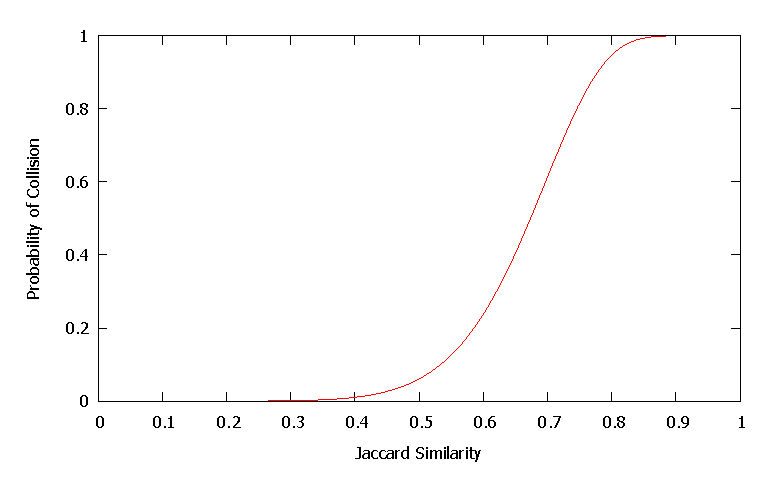
\epsfig{file=figures/scurve.eps, width=1.5in, height=1.3in}
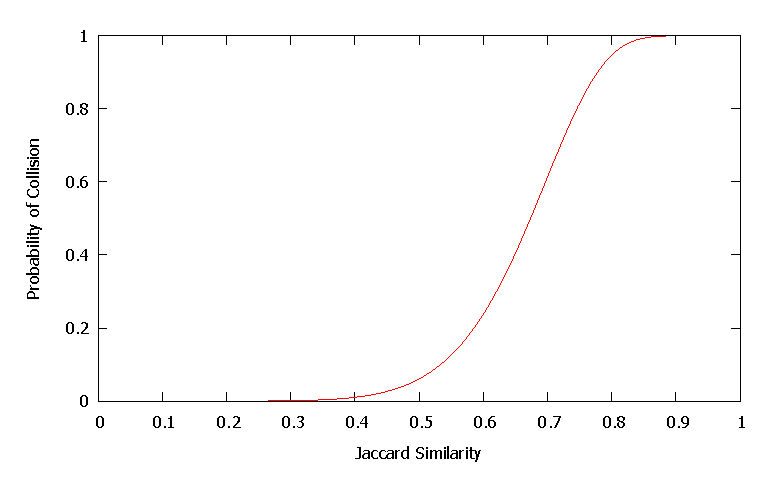
\includegraphics[width=1.5in, height=1.3in]{figures/scurve.eps}
\caption{$\Pr[\textnormal{Sig}(p)=\textnormal{Sig}(q)]=1-(1-d^r)^b$}
\label{fig:scurve}
\end{figure}
%The curve that Jaccard Similarity of two concept sets versus
%probability that their LSH signatures collide is illustrated in Figure
%\ref{fig:scurve}.



%We pre-compute LSH signatures for bid phrases' corresponding
%concept sets and build the LSH tables.
We pre-computed LSH signatures for all $p\in{}P$.%bid phrases' corresponding concept
%sets.
For each $i\in\{1,\ldots,b\}$, we firstly aggregate bid
phrases $P$ over $\text{Band}_{i}(p)$.
Then we maintain the index by a key-value pair memory object caching
system where the value of $\text{Band}_{i}(p)$ are used as keys and lists of
aggregated bid phrases are used as values.
We maintain the index of each band in one specific machine.
%inverted index by which, given the LSH signature
%of the given query's concept set, we can efficie-ntly retrieve bid
%phrases whose corresponding concept sets are mapped into the same
%buckets.
At runtime, when a query $q$ is posed, we compute its concept set's LSH
signature and distribute $\text{Band}_{i}(q),i=1,\ldots,b$ to corresponding machine
respectively.
%and use the signature to retrieve bid phrases through our hash tables.
For each band, we check whether $\text{Band}_{i}(q)$ happens to be
the key of a certain key-value pair.
If it is the case, value (i.e., list of bid phrases) of the pair is
considered because these bid phrases satisfies
$\text{Sig}(p)=\text{Sig}(p)$ and thus have large Jaccard similarity with
the $q$ under some probabilistic guarantee.
Bid phrases in that list are calculated exact Jaccard similarity with
respect to $q$ and we only return at most 100 true positive ones as
well as their Jaccard similarity value.
Finally, we merge results returned from the $b$ machines
and rank these bid phrases by their $\text{JS}(p,q)$ in descending
order.
The top 100 bid phrases (if we recalled enough) are selected as
candidates for the given $q$.


%True positive ones are selected as candidates.
%The disjunctive relationship between different bands enables us to
%process each of them seperately.
By the LSH scheme, we replace cumbersome calculation such as merging
hundreds of posting lists of inverted index by %several access to only
%a few hash tables.
accessing $b$ hash tables.
Besides, the scalability of our approach partly relies on the banding
technique because the disjunctive relationship between different bands enables
us to maintain each band in one machine and process in a parallel way.
It is this feature that improves the scalability and efficiency of our
system.
%Since these selected candidates are unordered.
%We rank them by computing their exact Jaccard Similarity with respect
%to query's concept set and rank them in descending order and only reserve
%at most about one hundred of them.
%The connection between short text and concepts can be modeled as a
%bipartite graph and organized in adjacent lists which can be stored in
%distributed key-value pair in-memory storage system(e.g., memcached)
%    easily when the scale of corpus is too large to be held in memory
%    of one machine.
\subsection{Ranking}
%In fact, we can simply rank candidates by Jaccard similarity between
%their concept sets and the given query's.  Since Probase is a
%probabilistic taxonomy, measuring similarity between concept sets only
%exploits its rich isA relationships but hasn't made full use of its
%typicalities.
We assign a semantic-matching score (SMS) to each candidate bid phrase
with respect to a given query.  Then we rank these candidates by their
assigned SMS score in descending order and select top ranking bid
phrases.  Intuitively, SMS should be proportional to the semantic
similarity between short texts.  Since each short text is
characterized by a concept vector, we can estimate the similarity
between short texts by measuring the similarity between their
corresponding concept vectors.  Formally, for a given query $q$ and a
bid phrase $p$, with their corresponding concept vectors denoted as
$\mathbf{c_q}$ and $\mathbf{c_p}$, SMS is defined as follows:
\begin{definition}
\begin{equation}
\textnormal{SMS}(q,p)=\cos(\mathbf{c_q},\mathbf{c_p})=\mathbf{c_q}\cdot\mathbf{c_p}
\end{equation}
\end{definition}
%By filtering a large portion of bid keywords and only reserving a
%handful of high-quality candidatas which seem to be relevant to given
%query, we can compute SMS for candidates with respect to given query
%in a meticulous way while satisfing the efficiency requirement of
%online system.\\
%
%
%
%Firstly, we distinguish head instances from tail instances to
%re-weight concepts derived from these observed instances.
%In contrast of classic term weighting scheme such as TF-IDF which
%measures significance of a word to a certain document based on the
%frequence of the word within the content of the document as well as
%the frequency of the word in the whole corpus, we determine the
%significance of each instance according to its functionality with
%respect to expressing the meaning of the short text.
%For example, short text ``angry birds for windows phone 7'' refers to
%the ``wp7'' version of a popular game named ``angry birds''. Here
%``angry birds'' is a head instance but ``windows phone 7'' is a modifier
%instance.
%By semantically re-weight associated concepts of each short text, we
%can target the core meaning of short text more accurately.
%We present our work on distinguishing head/modifier in another
%paper.
%
%
%
%Since taxonomy used in our approach organizes concepts hierarchically
%by ``is-A'' relation, regarding each concept as a independent
%coordinate and adopting conventional metrics(e.g., cosine) to measure
%similarity between two concept vectors seems unreasonable.
%Search users with identical search intent but different extent of
%expertise may issue different queries.
%For example, customer has no idea about ``kindle'' may issue query
%``amazon ebook reader'' and ``kindle'' is more specific but still so
%relevant to his/her query.
%In order to exploit more specific or more general bid phrases to
%answer given query, we measure similarity between short texts with
%consideration of not only their corresponding concept vector but also both their parent concepts and children concepts.
%Given a concept vector $\mathbf{c}$, we denote its corresponding
%concept set as
%$C_{\mathbf{x}}=\{(c_1,w_1),(c_2,w_2),\ldots,(c_n,w_n)\}$ where
%$\forall i\in 1,\ldots,n,w_i>0$.
%We derive parents of $C_{\mathbf{x}}$ by regarding concepts within it
%as entities and ranking their hypernyms by equation
%\ref{eqn:naivebayesian}.
%Children of $C_{\mathbf{x}}$ is derived by ranking hyponyms of its
%concepts by:
%\begin{equation}
%P(e\vert C_{\mathbf{x}})=\frac{P(e)P(C_{\mathbf{x}}\vert
%        e)}{P(C_{\mathbf{x}})}\propto P(e)\prod_{i}^{n}P(c_i\vert e)
%\end{equation}
%Then we transform parents and children of $C_{\mathbf{x}}$ into
%concept vector form and normalize them resulting
%$\mathbf{x}_{\textnormal{p}},\mathbf{x},\mathbf{x}_{\textnormal{c}}$.
%Given two concept vectors $\mathbf{x}$ and $\mathbf{y}$, we define the
%SMS of them as:
%\begin{definition}
%SMS($\mathbf{x},\mathbf{y}$)=$\max_{t\in\{\mathbf{x}_{\textnormal{p}},\mathbf{x},\mathbf{x}_{\textnormal{c}}\}\times\{\mathbf{y}_{\textnormal{p}},\mathbf{y},\mathbf{y}_{\textnormal{c}}\}}\cos(t)$
%\end{definition}


%%% Local Variables:
%%% mode: latex
%%% TeX-master: "adselection"
%%% End:

%\section{Ranking Function}
In this module, we assign semantic-matching score(SMS) to each
candidate with respect to given query.
Then we rank these candidates by assigned score in descending order
and select top rank bid keywords as resulting substitution/expansion
for given query.
The SMS should reveal the semantic similarity between short texts.
By filtering a large portion of bid keywords and only reserving a
handful of high-quality candidatas which seem to be relevant to given
query, we can compute SMS for candidates with respect to given query
in a meticulous way while satisfing the efficiency requirement of
online system.\\
Firstly, we distinguish head instances from tail instances to
re-weight concepts derived from these observed instances.
In contrast of classic term weighting scheme such as TF-IDF which
measures significance of a word to a certain document based on the
frequence of the word within the content of the document as well as
the frequency of the word in the whole corpus, we determine the
significance of each instance according to its functionality with
respect to expressing the meaning of the short text.
For example, short text ``angry birds for windows phone 7'' refers to
the ``wp7'' version of a popular game named ``angry birds''. Here
``angry birds'' is a head instance but ``windows phone 7'' is a modifier
instance.
By semantically re-weight associated concepts of each short text, we
can target the core meaning of short text more accurately.
We present our work on distinguishing head/modifier in another
paper.\\
%Since taxonomy used in our approach organizes concepts hierarchically
%by ``is-A'' relation, regarding each concept as a independent
%coordinate and adopting conventional metrics(e.g., cosine) to measure
%similarity between two concept vectors seems unreasonable.
Search users with identical search intent but different extent of
expertise may issue different queries.
For example, customer has no idea about ``kindle'' may issue query
``amazon ebook reader'' and ``kindle'' is more specific but still so
relevant to his/her query.
In order to exploit more specific or more general bid keywords to
answer given query, we measure similarity between concept vectors with
consideration of both their parent concepts and children concepts.
Given a concept vector $\mathbf{x}$, we denote its corresponding
concept set as
$C_{\mathbf{x}}=\{(c_1,w_1),(c_2,w_2),\ldots,(c_n,w_n)\}$ where
$\forall i\in 1,\ldots,n,w_i>0$.
We derive parents of $C_{\mathbf{x}}$ by regarding concepts within it
as entities and ranking their hypernyms by equation
\ref{eqn:naivebayesian}.
Children of $C_{\mathbf{x}}$ is derived by ranking hyponyms of its
concepts by:
\begin{equation}
P(e\vert C_{\mathbf{x}})=\frac{P(e)P(C_{\mathbf{x}}\vert
        e)}{P(C_{\mathbf{x}})}\propto P(e)\prod_{i}^{n}P(c_i\vert e)
\end{equation}
Then we transform parents and children of $C_{\mathbf{x}}$ into
concept vector form and normalize them resulting
$\mathbf{x}_{\textnormal{p}},\mathbf{x},\mathbf{x}_{\textnormal{c}}$.
Given two concept vectors $\mathbf{x}$ and $\mathbf{y}$, we define the
SMS of them as:
\begin{definition}
SMS($\mathbf{x},\mathbf{y}$)=$\max_{t\in\{\mathbf{x}_{\textnormal{p}},\mathbf{x},\mathbf{x}_{\textnormal{c}}\}\times\{\mathbf{y}_{\textnormal{p}},\mathbf{y},\mathbf{y}_{\textnormal{c}}\}}\cos(t)$
\end{definition}

%\section{Flight Analysis}
In reality, search engine preprocesses a list of queries offline and
builds inverted index for the resulting expansions(query as term and
    its expansion as corresponding posting list).
At runtime, search engine uses the resulting expansions to find
relevant bid keywords for submitted query.
When there is enough traffic volumne to ensure computed metrics(e.g.,
        click through rate(CTR), cost per click(CPC), etc.) reliable,
     search engine will analysis and prune those bad expansion.
For example, a certain bid keyword is high-ranking in the expansion
for a certain query.
However, the CTR for ads retrieved through this bid keyword is so low.
This bid keyword may be not so relevant to that query and search
engine will eliminate it from that query's expansion in the next
version.
Although pruning is not an elegant approach to improve effectiveness
of sponsored search, it is an important and indespensable step of
sponsored search adopted by many mainstream search engines.\\
Different from latent semantic analysis approaches which represent
documents as distribution over latent topics and topics as
distributions over vocabulary of indexed corpus, our approach
represents documents as explicit topics where topics are concepts used
in our daily life.
Such a representation representation of the meaning behind any text is
easy to explain to human users\cite{gabrilovich:semanticanalysis}.
By our explicit representation of semantic meaning, we are able to not
only prune resulting expansion based on conventioinal metrics but also
infer and analysis more detailed problem behind the sympton such as
which topics(concepts) contain commercial intent, which domains our
approach can't not generate useful expansions.
For example, when we find that CTRs of expansions for queries related
to concept ``hotel'' are lower than other topics(concepts).
We can collect these queries and design vertical search engine for
this specific domain.


\section{Experiment}
%We designed and implemented a series of experiments to evaluate the
%performance of our approach.
This section describes the experiment settings and analyses the
experiment results.
Experiments described in this section mainly made use of the following
data:
\begin{itemize}
\item \textbf{Keyword set:} a massive dataset consisting of 0.702
billion bid phrases.
\item \textbf{Query set:} a collection of 30 million search queries.
\item \textbf{Search logs:} 15.5 billions of records of the
form: <query:str, bid phrase:str, $\ldots$, click-or-not:bool> within
which there exist 0.83 billion distinct queries.
\end{itemize}
All these data are provided by a commercial search engine and the
search log is accumulated during one month period of time.
%We firstly checked the effectiveness of proposed disambiguation
%approach.
%After conceptualization, bid phrases are mapped into our concept space.
%To expand a query, we firstly select candidate bid phrases for it.
%So experiment is made to comparison between our candidates
%selection approaches (i.e., CSCD and CSJS).
%%We estimate the similarity between each candidate with a given query by
%%SMS.
%Then candidates are ranked based on SMS.
%Thus, we evaluated SMS before assessing the resulting suggestions
%(expansions) of a given query.
%%In our third experiment, we observed a
%%strong positvie correlation between SMS and search users' interests.
%Finally, to show that proposed approach is effective for query
%expansion and keyword suggestion, we assessed the relevance between
%retrieved bid phrases and the given queries.
    %We designed and implemented the following experiments to examine the
%performance of our approach:
%\begin{enumerate}
%\item We begin evaluating our approach with semantic-matching score(SMS).
%%We assign SMS to each candidate bid phrase based on similarity between
%it and given query.
%\item we evaluate the quality of retrieved bid phrases.
%%In contrast to traditional IR which only focuses on the relevance
%%between retrieved documents and given query, we prefer to bid phrases
%%which are not obvious yet relevant.
%\item We make comparison between candidates selection approaches
%proposed in this paper.
%\end{enumerate}
%To prove the efficacy of semantic-matching score proposed in our
%approach, we mined click-through data to evaluate the correlationship
%between CTR and computed semantic-matching score.
%We sampled several queries from search log and generated expansion for
%them using both traditional term matching scheme and our approach.
%User study was held to compare the quality of resulting expansions.
%We also compared the performance of different candidates selection
%approaches proposed in this paper on specific domain.
%Finally, we report the result of flight analysis supported by Bing
%search engine.
%It not only reveals the scalability and efficiency of our approach,
%   but also a more credible evaluation for effectiveness.
\subsection{Disambiguation}
With rich isA relationships, knowledge-based approaches can map
terms to their synonyms and similar varieties through their hypernyms.
However, existing approaches neglected polysemy which is also
prevalent especially within bid phrases. We have emphasized that
leveraging our co-occurrence network, we can identify the appropriate
sense of detected instnace, so we made experiment to evaluate the
effect of our disambiguation approach.


We randomly sampled one million bid phrases from our keyword set and
then extracted those containing ambiguous instances ``apple'',
     ``blackberry'', ``palm'', ``bass'' and ``mouse'' as our test set.
We applied our approach to conceptualize each of these bid phrases.
Thus each occurrence of the five ambiguous instances is explicitely
associated with one of its sense.
Regarding the disambiguation as a classification problem, we manually
labeled correct sense for these ambiguous instances appeared in test
set and adopted accuracy as metrics to access the effect of our
disambiguation approach.


The experiment results are presented in Table \ref{tab:acc}. The
classification accuracy of ``bass'' seems not satisfiable because
multi-class classification is much more tough in most cases. Most of
the miss classified samples of ``apple'' are those which refer to
``tree'' but associated with ``fruit'' and vice versa. The reason is
that seperating these two senses from ``company'' is easy but the two
senses themselves are somehow similar. It is more difficult to
identify the proper sense under a smaller granularity.
\begin{table}
\centering
\begin{tabular}{|c|c|c|c|c|}\hline
instance&\#senses&\#correct&\#sample&accuracy\\\hline
apple&3&157&171&0.918\\\hline
blackberry&2&127&142&0.894\\\hline
palm&3&76&84&0.905\\\hline
bass&4&46&57&0.807\\\hline
mouse&2&184&200&0.920\\\hline
\end{tabular}
\caption{Accuracy of disambiguation}
\label{tab:acc}
\end{table}
\subsection{CSCD v.s. CSJS}
%\subsection{Candidates Selection Comparison}
\textbf{Objective} of this experiment is to compare the two candidates
selection approaches proposed in this paper.
%Although Probase is full of common sense knowledge which can be used
%for general purpose task and approach proposed in our paper is
%intended to resolve open-domain keyword suggestion and query expansion.
The CSCD (see Subsection \ref{sec:CSCD}) mines click-through data to
extract co-click relationships between queries.
Although the co-click relationships capture semantic relatedness
between queries accurately, there are inadequate click-through data for
tail queries.
Thus, CSCD can't be applied for tail queries.
On the other hand, CSJS (see Subsection \ref{sec:CSJS}) directly
leverages semantic knowledge provided by Probase and thus has broader
application scenarios than CSCD.


\textbf{Dataset} used for this experiment includes our keyword set as
well as 21 queries randomly sampled from our search logs.
These queries are all related to a specific domain---``hotel''.
%Thus, we compare the two different candidates selection
%approaches---CSCD and CSJS(see subsection \ref{sec:CSJS}) using queries all belong to a very popular
%topic---``hotel''.
%It is still meaningful for us to evaluate the performance of our
%approach for queries of a specific domain especially popular
%topics(e.g., travel, hotel, insurance, etc.) because search engines
%usually provide vertical search engines for them which are designed
%for a certain specific domain and usually achieve better
%performance on their corresponding domain compared with general
%purpose approach.
%We randomly sampled 21 queries from search log which are all related
%to ``hotel'' topic.
Because ``hotel'' is one of the three most popular topics(i.e.,
        ``travel'', ``hotel'', ``insurance'') of sponsored search,
        there is sufficient click information for these sampled
        queries, and thus CSCD can perform well for them.


For each sampled query, we ranked candidate bid phrases that are
selected by CSCD and CSJS respectively based on SMS and reserved at
most top-$30$ as retrieval results.
%We select relevant bid phrases for sampled queries from 702 millions
%of bid phrases contained by a commercial search engine using framework
%proposed in this paper while different candidates selection approaches.



\textbf{Metrics} used for accessing retrieved results %of the two
%approaches
is average precision at N (\emph{P@n})
    \cite{baeza2011modern}.
We manually labeled more than 1200 query-bid phrase pairs
according to the labeling guideline listed in Table
\ref{tab:scoringrule}.
We computed P@n by regarding bid phrases with score 1 or 2 as
good(positive) cases, and average \emph{``extreme''} precision at n by
regarding only bid phrases with score 2 as good(positive) cases.
\begin{table}
\centering
\begin{tabular}{|c|c|}\hline
Score (Label)&Reasons\\\hline
2 point      &Synonymy;Word Permutation;\\
very relevant&CAL;Disambiguation.\\\hline
1 point&Subset;Overlap;\\
somewhat relevant&Superset;Similar.\\\hline
0 point   &Clarion hotels$\rightarrow$\\
Irrelevant&hotels rewards cards\\
\hline
\end{tabular}
\caption{Labeling Guideline for Hotel Queries and Bid Keywords}
\label{tab:scoringrule}
\end{table}
%We also compare different candidates selection approaches.
%Selection by measuring Jaccard Similarity and Overlap Similarity is
%denoted as Approach\uppercase\expandafter{\romannumeral1} while
%selection by exploiting co-click information is denoted as Approach\uppercase\expandafter{\romannumeral2}.
\begin{table}[!ht]
\centering
\begin{tabular}{|p{2cm}|c|c|c|c|}
\hline
label&\multicolumn{2}{|c|}{CSJS}&\multicolumn{2}{|c|}{CSCD}\\
\cline{2-5}
     &\#count&ratio&\#count&ratio\\
\hline
0&15&0.062&2&0.010\\
\hline
1&174&0.719&90&0.429\\
\hline
2&53&0.219&118&0.562\\
\hline
P@10&\multicolumn{2}{|c|}{93.80\%}&\multicolumn{2}{|c|}{99.05\%}\\
\hline
extreme P@10&\multicolumn{2}{|c|}{21.90\%}&\multicolumn{2}{|c|}{56.19\%}\\
\hline
\end{tabular}
\caption{P@10 of CSJS and CSCD}
\label{tab:pat10}
\end{table}
\begin{table}[!h]
\centering
\begin{tabular}{|p{2cm}|c|c|c|c|}
\hline
label&\multicolumn{2}{|c|}{CSJS}&\multicolumn{2}{|c|}{CSCD}\\
\cline{2-5}
     &\#count&ratio&\#count&ratio\\
\hline
0&38&0.082&3&0.007\\
\hline
1&332&0.719&196&0.467\\
\hline
2&92&0.199&221&0.526\\
\hline
P@20&\multicolumn{2}{|c|}{91.77\%}&\multicolumn{2}{|c|}{99.29\%}\\
\hline
extreme P@20&\multicolumn{2}{|c|}{19.91\%}&\multicolumn{2}{|c|}{56.62\%}\\
\hline
\end{tabular}
\caption{P@20 of CSJS and CSCD}
\label{tab:pat20}
\end{table}



\textbf{Experiment results} are illustrated in Table \ref{tab:pat10} and
Table \ref{tab:pat20}.
%Approach\uppercase\expandafter{\romannumeral1}
As you can see, CSCD outperforms CSJS which confirms the intuition that
co-click relationships can accurately capture semantic relatedness.
%\uppercase\expandafter{\romannumeral2}.
%It benefits from click-through data which provide useful hints for
%selecting highly relevant bid phrases as candidates.
However, not all topics are as popular as ``hotel''.
%In many cases, queries related to rare topics are seldom accessed
%by search users.
When there is no sufficient click-through data for CSCD to draw
reliable conclusions, CSJS will function as CSCD's complement.
\subsection{Validating Semantic-Matching Score}
%Ranking function assigns scores to documents with regard to a given query~\cite{baeza2011modern}.
%Our approach is of no exception.
%We assigned \emph{SMS} to each bid phrase with respect to a given
%query.
We ranked candidate bid phrases by \emph{SMS} and select the
top-ranking ones as resulting expansions for the issued query.
Obviously, only when SMS reflects the relevance between short texts
accurately can we rank bid phrases in a reasonable order.
\subsubsection{Ground Truth}
As we know, click thorugh rate (\emph{CTR}) of an ad is defined as the
number of clicks on this ad divided by the number of the ad's
impressions.
High CTR indicates successful advertising campaign.
Because the matching of query to ads is through bid phrases, we can
apply CTR for bid phrases by simply accumulating impressions according
to bid phrases instead of ads.
Accordingly, we define CTR of query-bid phrase pair as follow:
\begin{definition}
\label{def:ctr}
Given query $q$ and bid phrase $p$, we have
\begin{equation}
\text{CTR}(q,p)=\frac{\text{Clicks}(q,p)}{\text{Impressions}(q,p)}\times
100\%
\end{equation}
where both clicks and impressions are triggered by bid phrase $p$ in
response to query $q$.
\end{definition}
We extracted tuples in the form $<query:string, bid
    phrase:string, click-or-not:bool>$ from our search logs.
Then we computed CTR of each query-bid phrase pair by aggregating all
these tuples over their first two columns.



%Then we can use CTR of query-bid keyword pair as the actual similarity
%or at least a high-quality approximation of similarity between the
%query and bid keyword.
%So we can check that whether semantic-matching score makes sense in
%terms of representing the similarity between short text by analysing
%the correlation between CTR and it.
We made assumption that CTR of query-bid phrse pair is proportional to
their semantic similarity and used CTR as ground truth.
Thus, to check whether SMS properly reveals semantic similarity between short
texts, we check whether there exists a strong positive correlation
between SMS and CTR.
In another word, if higher SMS corresponds to higher CTR and lower SMS
corresponds to lower CTR, we have confidence to announce that SMS can
reflect semantic similarity between short texts accurately.
\subsubsection{SMS v.s. CTR}
We quantitate SMS evenly into ten intervals denoted by integral
identifiers ranging from 1 to 10 where interval with larger identifier
corresponds to higher SMS.
To observe the relationship between SMS and CTR, we present Figure
\ref{fig*:subfig:a}.
Horizontal axis of it represents the identifiers of SMS intervals.
%semantic-matching score of query-bid keyword pair. We quantitate it
%into ten buckets denoted by integers from 1 to 10 where larger integer
%means higher semantic-matching score.
Vertical axis of it represents the average CTR of query-bid phrase
pairs.
As you can see, pairs with higher SMS have higher CTR.
There exists a strong positive correlation between them which persuasively
proves the effectiveness of SMS.
%Although the number of impressions does not increase monotonically.
%It overall also reveals strong correlation with semantic-matching
%score.
\begin{figure*}[!t]
    \subfigure[Different SMS Range] {
        \label{fig*:subfig:a}
        \begin{minipage}[b]{0.33\textwidth}
            \centering
            %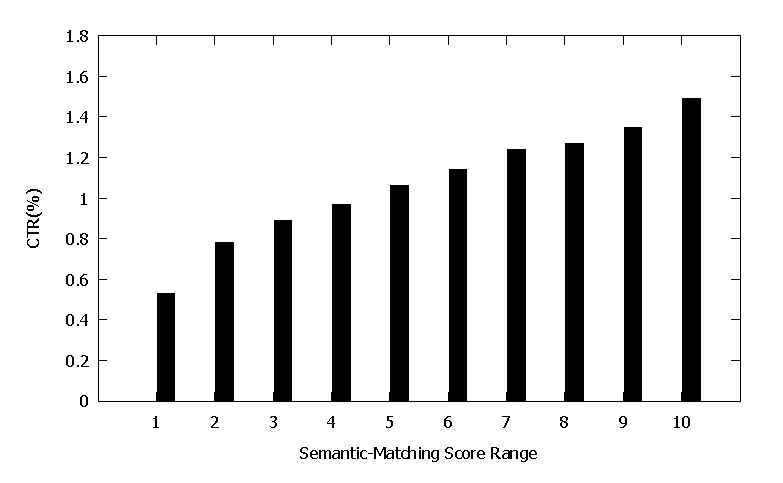
\epsfig{file=figures/correlation.eps,height=1.2in,width=2.2in}
            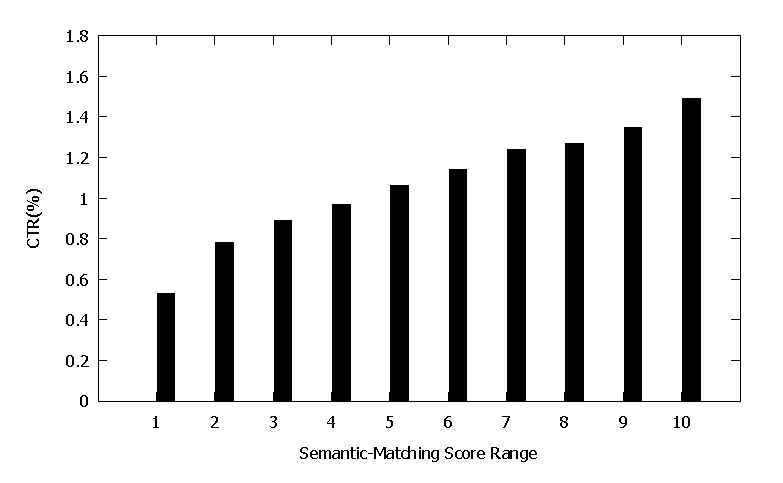
\includegraphics[height=1.2in,
                width=2.2in]{figures/correlation.eps}
        \end{minipage}}%\vspace{-1.0mm}
    \subfigure[Head Queries] {
            \label{fig*:subfig:b}
            \begin{minipage}[b]{0.33\textwidth}
            \centering
            %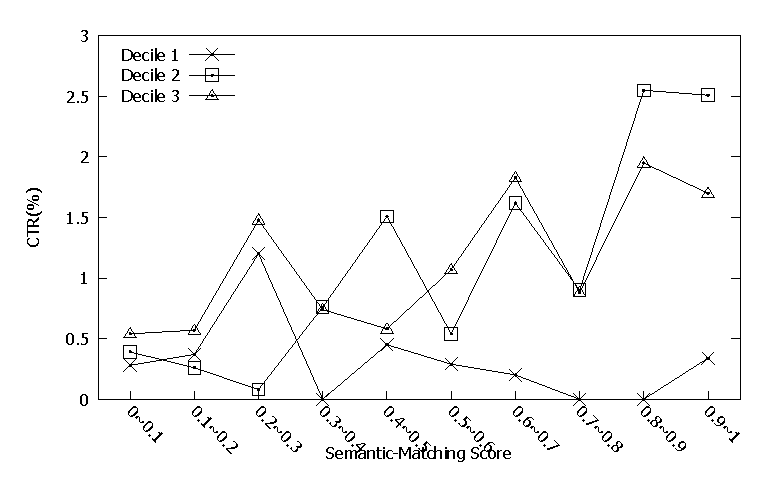
\epsfig{file=figures/headdecile.eps,height=1.2in,width=2.2in}
            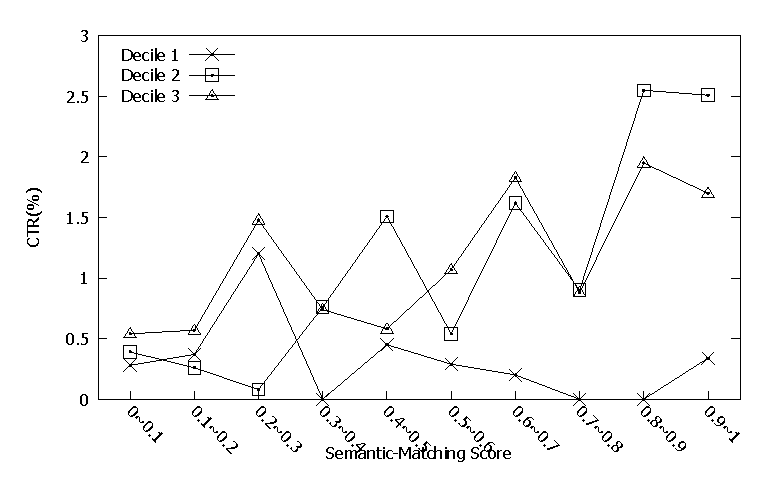
\includegraphics[height=1.2in,
                width=2.2in]{figures/headdecile.eps}
        \end{minipage}}%\vspace{-1.0mm}
    \subfigure[Torso Queries] {
            \label{fig*:subfig:c}
            \begin{minipage}[b]{0.33\textwidth}
            %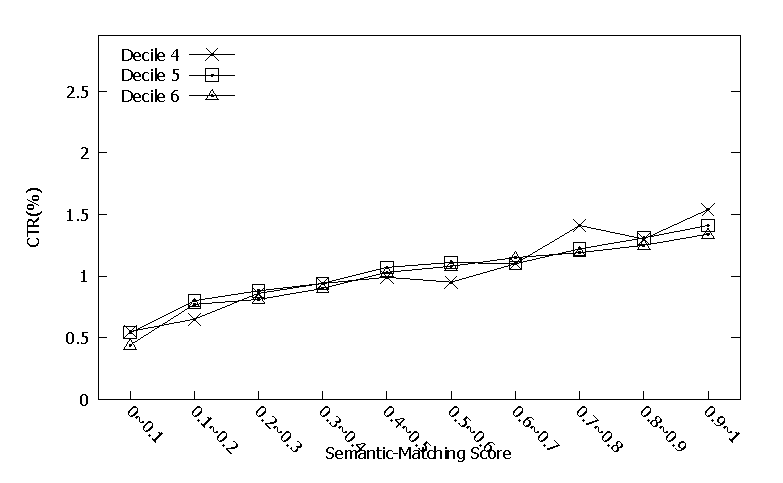
\epsfig{file=figures/torsodecile.eps,height=1.2in,width=2.2in}
            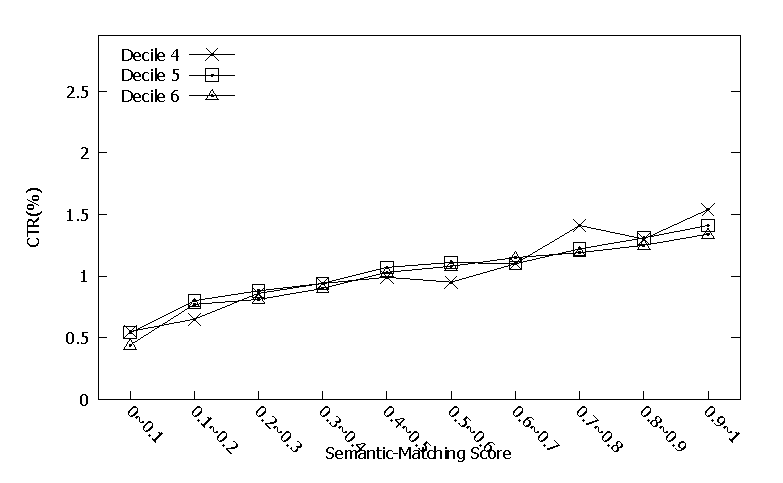
\includegraphics[height=1.2in,
                width=2.2in]{figures/torsodecile.eps}
        \end{minipage}}\\
    \subfigure[Tail Queries] {
        \label{fig*:subfig:d}
        \begin{minipage}[b]{0.33\textwidth}
        \centering
            %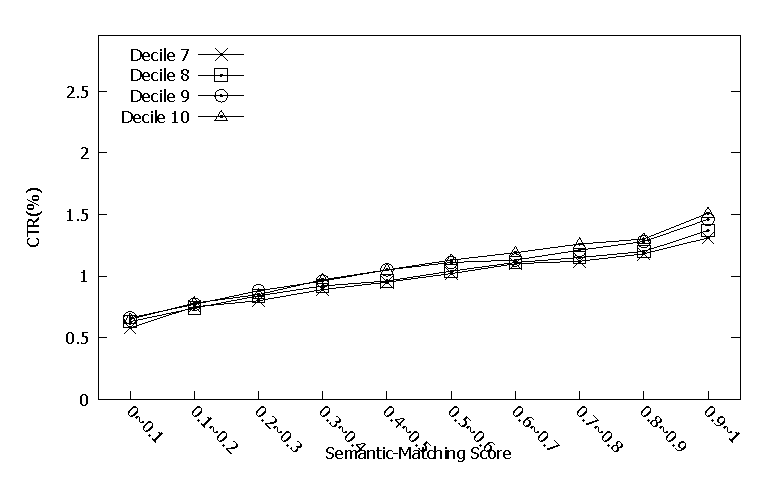
\epsfig{file=figures/taildecile.eps,height=1.2in,width=2.2in}
            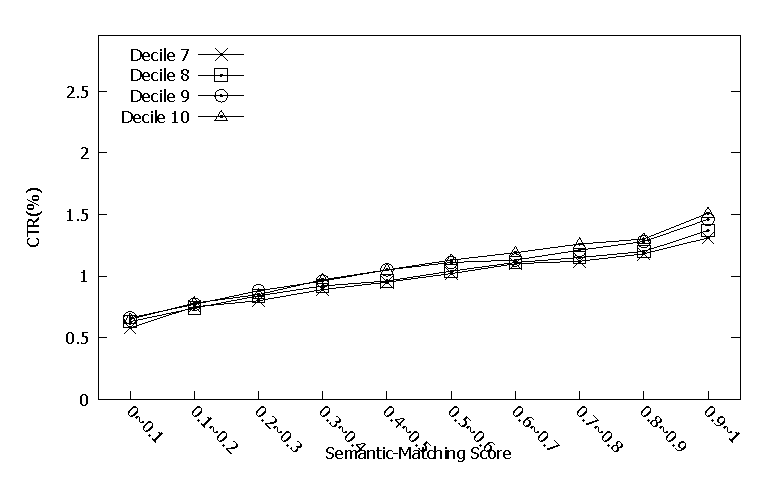
\includegraphics[height=1.2in,
                width=2.2in]{figures/taildecile.eps}
        \end{minipage}}%\vspace{-1.0mm}
    \subfigure[Mainline Ads] {
        \label{fig*:subfig:e}
        \begin{minipage}[b]{0.33\textwidth}
        \centering
            %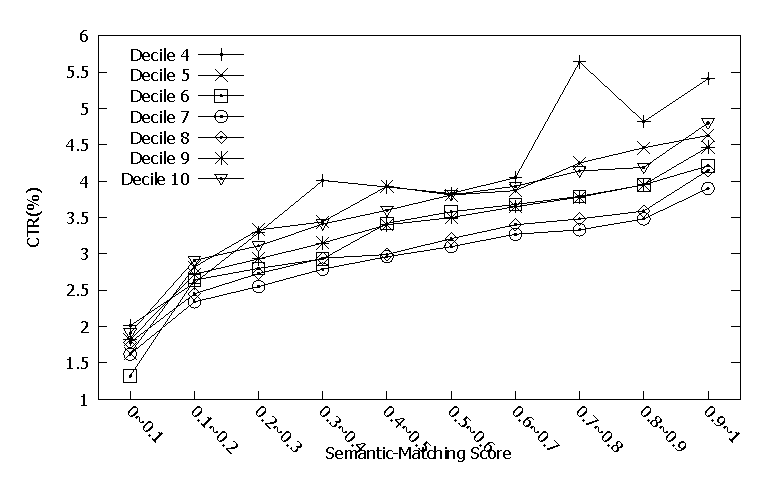
\epsfig{file=figures/ml.eps,height=1.2in,width=2.2in}
            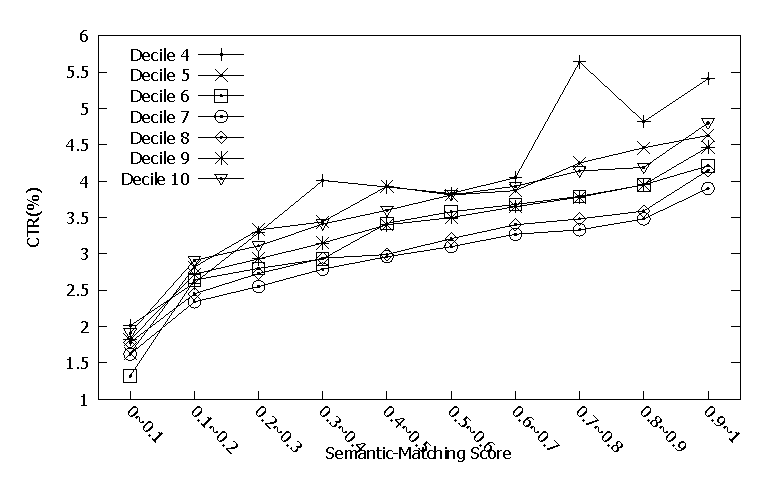
\includegraphics[height=1.2in,
                width=2.2in]{figures/ml.eps}
        \end{minipage}}
    \subfigure[Sidebar Ads] {
        \label{fig*:subfig:f}
        \begin{minipage}[b]{0.33\textwidth}
        \centering
            %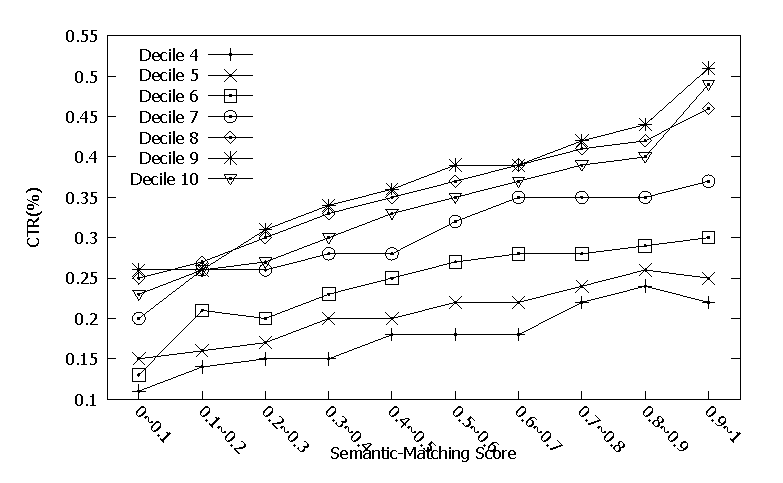
\epsfig{file=figures/sb.eps,height=1.2in,width=2.2in}
            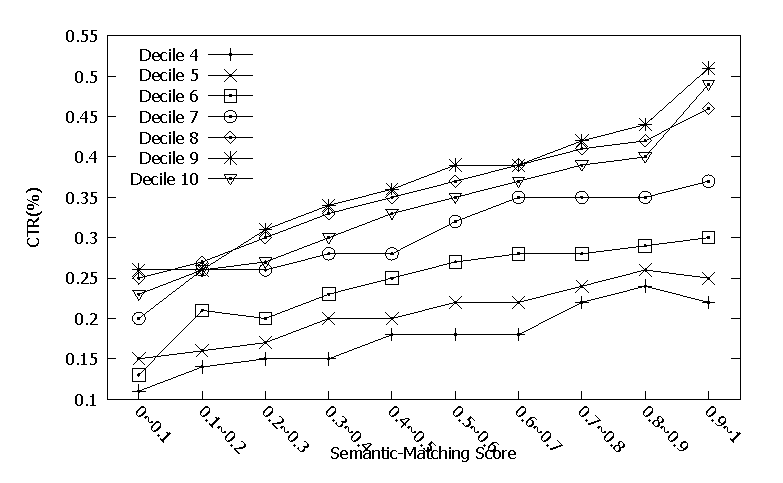
\includegraphics[height=1.2in,
                width=2.2in]{figures/sb.eps}
        \end{minipage}}
    \caption{Correlation between Semantic-Matching Score and CTR}
    \label{fig*:ex1}
\end{figure*}



It is well known that the volume distribution of search queries
follows the power law~\cite{broder:sponsoredsearch}.
We divide the query volume into ten deciles evenly. %in which they have the same total volume of traffic.
\begin{itemize}
\item \emph{Head queries} belong to deciles $1\sim 3$.
They are extremely popular and searched frequently.
\item \emph{Torso queries} belong to deciles $4\sim 6$.
\item \emph{Tail queries} belong to deciles $7\sim 10$.
These queries are rarely accessed and thus have limited historical
data.
\end{itemize}
%Then the frequently accessed queries belong to classes with lower
%decile value while torso and tail queries belong to classes with
%higher decile value.
We show the relationships between SMS and CTR of query-bid phrase pair
for head, torso and tail queries in Figure \ref{fig*:subfig:b},
    \ref{fig*:subfig:c}, \ref{fig*:subfig:d} respectively.
Although SMS fails to reveal the semantic similarity between head
queries and bid phrases accurately, both keyword suggestion and query
expansion for these popular queries have been resolved well.
Consequently, we can leverage co-click signals described in subsection \ref{sec:CSCD} for head queries.
As you can see, for torso and tail queries, there exists a strong
positive correlation between SMS and CTR of query-bid phrase pair, which
confirms the effectiveness of SMS.
Because these queries lack of user behavior data, they can't be covered
by most existing approaches and are research topics of this area.
%By employing semantic knowledge to resolve the bottleneck, our
%approach is helpful for current search engines.



\subsubsection{Ranking by SMS}
\label{sec:smsrank}
\textbf{Objective} of this experiment is to check whether the ranking
determined by SMS is reasonable.
Although the strong correlation between SMS and CTR confirms the effectiveness
of SMS,
%proves that scores assigned
%to bid phrases with regard to a given query are reasonable.
%However, 
    gathering such statistic(i.e., CTR) globally may fail to distinct an
approach that ranks highly relevant bid phrases at the top from
another approach that ranks mildly relevant bid phrases at the top.
%We will take the \emph{order} into consideration in this experiment.
%To show that our approach has the ability to generate reasonable
%ranking for retrieved bid keywords at the top of the result, we
%compare our approach against other mainstream approaches on a dataset
%sampled from search log with Normalized Discounted Cumulated
%Gain(NDCG) as metrics.



\textbf{Dataset} for this experiment are
%search logs accumulated
%during one month period of time by a commercial search engine.
%The search logs consist of about 15.5 billion records within which
%there exist 0.83 billion distinct queries.
%From these search logs, we randomly choose
2504 queries(1000 head
        queries, 1000 torso queries and 504 tail queries) randomly
sampled from our search logs.
Firstly, we computed CTR of query-bid phrase pair for these sampled
queries.
Then we rank each query's bid phrases by their CTRs in descending
order and reserve the top 30 ones (there are only 504 tail queries that
        contain at least 30 bid phrases).
The ranking as well as these bid phrases' CTRs are used as ground
truth for this experiment.



%Since there are a few cases where queries are so relevant to bid
%keywords which are not within their corresponding CTR rank and we don't
%want to revise our dataset manually to avoid loss of objectivity, 
\textbf{Metrics} should take the ranking orders of retrieved bid
phrases into account so that more reasonable rankings can be
distinguished from unreasonable ones.
Thus, we choose Normalized Discounted Cumulated Gain(\emph{NDCG}~\cite{baeza2011modern}) as
    our metrics.
Given a sampled query $q$, aggregate records of search logs to compute
CTR of bid phrases with respect to $q$.
Then we rank bid phrases associates with $q$ by their CTR and reserve
the top 30 bid phrases $(p_{1},\ldots,p_{30})$.
%$(p_{1},\textnormal{CTR}(q,p_1)),\ldots,(p_{30},\textnormal{CTR}(q,p_{30}))$.
We compute the Ideal Discounted Cumulated Gain
(\emph{IDCG}~\cite{baeza2011modern}) of $q$ by
\begin{equation}
\textnormal{IDCG}(q)=\textnormal{CTR}(q,p_1)+\sum_{i=2}^{30}\frac{\textnormal{CTR}(q,p_i)}{\log_{2}i}
\end{equation}
If we rank the top 30 bid phrases of $q$ by some approach, we derive
$p_{f(1)},\ldots,p_{f(30)}$.
Then we compute the Discounted Cumulated Gain (\emph{DCG}~\cite{baeza2011modern}) by
\begin{equation}
\textnormal{DCG}(q)=\textnormal{CTR}(q,p_{f(1)})+\sum_{i=2}^{30}\frac{\textnormal{CTR}(q,p_{f(i)})}{\log_{2}i}
\end{equation}
Finally, NDCG of $q$ can be computed by
\begin{equation}
\textnormal{NDCG}(q)=\frac{\textnormal{DCG}(q)}{\textnormal{IDCG}(q)}
\end{equation}
%The NDCG is defined as %    devided by Ideal Discounted Cumulated Gain(\emph{IDCG}).
%we compute NDCG for each query by ranking the corresponding CTR
%rank of it using CTR value as gain and original CTR rank as ideal
%order to compute Ideal Discounted Cumulated Gain (IDCG).



\textbf{Baselines} include bag-of-words technique,
    pLSA~\cite{hofmann:semanticindexing} and
    ESA~\cite{gabrilovich:semanticanalysis}.
We weight terms using classic TF-IDF scheme and set the number of
topics of pLSA to 100.
TF-IDF weights and probabilities of pLSA model are estimated with
respect to all sampled queries as well as their bid phrases.
%Because bid phrase that has no common terms with its corresponding
%query will not be recalled by bag-of-words technique, we discard such
%kind of bid phrases in re-ranked list.



\begin{figure*}[!ht]
    \subfigure[NDCG on head queries] {
        \label{fig:subfig:a1}
        \begin{minipage}[b]{0.33\textwidth}
            \centering
            %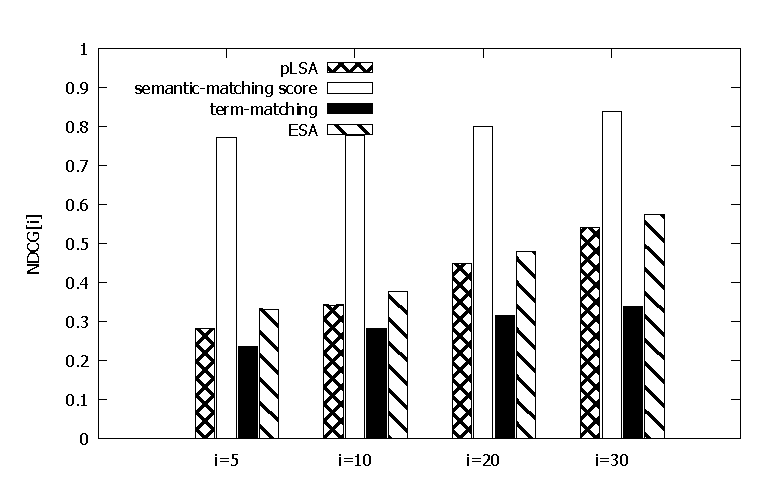
\epsfig{file=figures/headndcg.eps,height=1.2in,width=2.2in}
            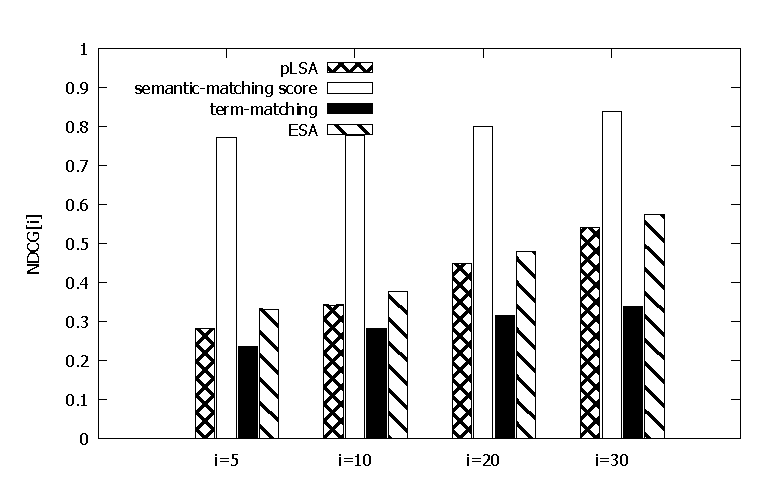
\includegraphics[height=1.2in,
                width=2.2in]{figures/headndcg.eps}
        \end{minipage}
    }
    \subfigure[NDCG on torso queries] {
        \label{fig:subfig:b1}
        \begin{minipage}[b]{0.33\textwidth}
            \centering
            %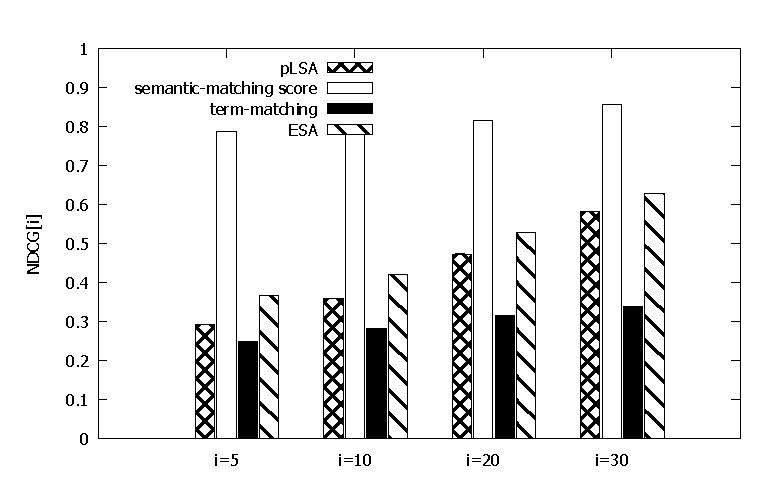
\epsfig{file=figures/torsondcg.eps,height=1.2in,width=2.2in}
            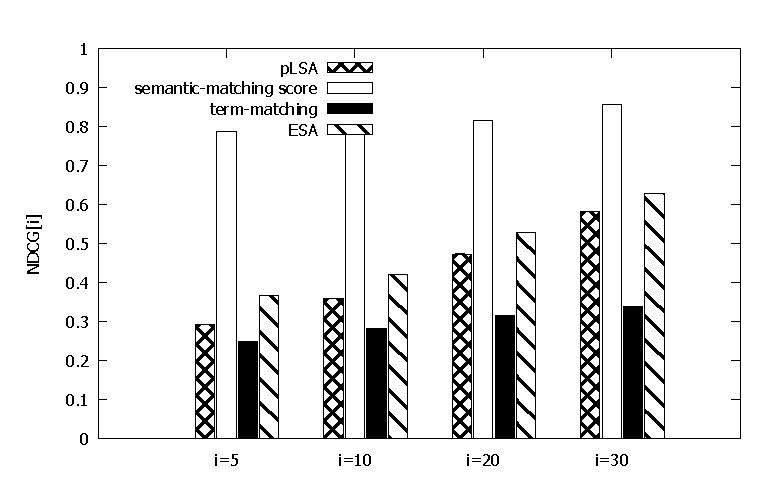
\includegraphics[height=1.2in,
                width=2.2in]{figures/torsondcg.eps}
        \end{minipage}
    }
    \subfigure[NDCG on tail queries] {
        \label{fig:subfig:c1}
        \begin{minipage}[b]{0.33\textwidth}
            \centering
            %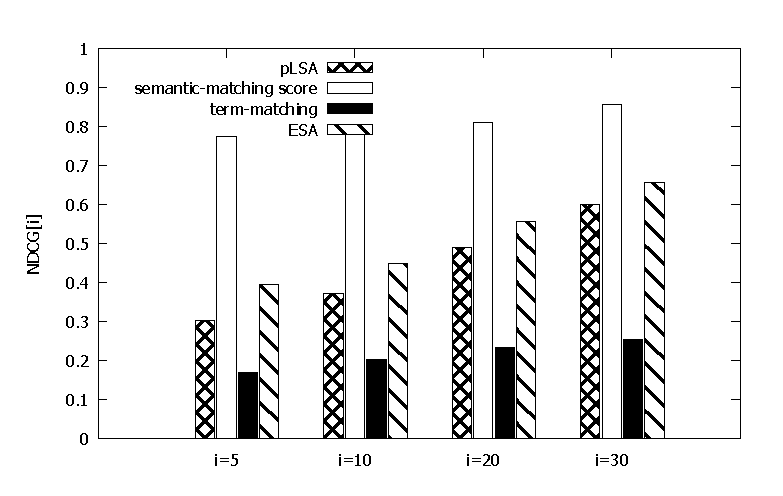
\epsfig{file=figures/tailndcg.eps,height=1.2in,width=2.2in}
            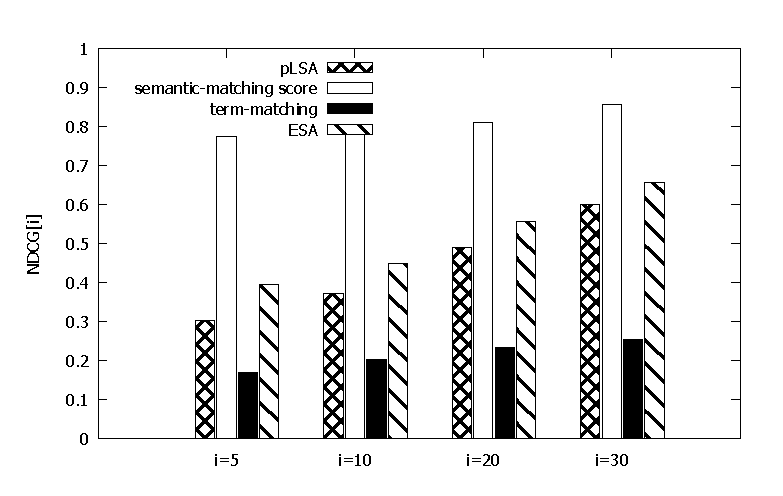
\includegraphics[height=1.2in,
                width=2.2in]{figures/tailndcg.eps}
        \end{minipage}
    }
    \caption{NDCG}
    \label{fig*:ndcg}
\end{figure*}
\textbf{Experiment results} are illustrated in Figure \ref{fig*:ndcg}.
Our approach outperforms baselines under all kinds of settings.
Bag-of-words technique can't recall sufficient bid phrases so it
loses many bid phrases' ``gains'' and results in low NDCG.
Bid phrases' distributions over latent topics are extremely sparse
because each bid phrase contains limited words.
Both ESA and our approach model short texts as explicit concepts and
thus reveal satisfactory coverage and accuracy.
Our approach beats ESA mainly because of the different strategies of
conceptualization.
ESA maps short text into wikipedia's concept space based on
co-occurrence of terms within the short text itself and terms of 
concepts' corresponding articles.
We associate short texts with relevant concepts according to entities
of them.
Since both queries and bid phrases are very short, conceptualization
directly via \emph{isA} relationship is more robust than strategy of
ESA.
\subsection{Retrieval Evaluation}
%Our approach is tasked with selecting relevant bid phrases from a
%massive corpus with respect to a given query.
Approach proposed in this paper intends to match a given query to
relevant bid phrases.
%The resulting bid phrases are retrieved from a extremely huge corpus.
Although previous experiment has confirmed the effectiveness of SMS,
         ranking a small set of bid phrases in a reasonable order is
         only a subproblem of retrieving relevant ones from a
         extremely huge corpus.
Evaluation from the standard IR perspective is indispensable.
\subsubsection{Comparison with Existing Approaches}
\textbf{Dataset} for our evaluation purpose includes a set of testing
queries and a corpus of bid phrases.
We randomly sampled 2554 queries from our search logs as testing
queries.
%sampled from search logs mentioned in Section \ref{sec:smsrank}.
%as our test queries.
%These search logs are accumulated during one month period of time.
%They consist of about 15.5 billion records within
%which there are around 0.83 billion distinct queries.
We also sampled 300,000 bid phrases from our keyword set which have no
common term with our testing queries.
We treat these bid phrases as negative (not relevant) cases if they
appear in the retrieval results of any test query.
Contemporary commercial search engines provide keyword search tools
for advertisers to expand a given query with a list of highly relevant
bid phrases.
%To save labour, we compare our approach with several baselines using
%bid phrases expanded by keyword search tool of a commercial
%search engine.
We make use of keyword search tool provided by a commercial search
engine to expanded our test queries.
%In fact, this keyword search tool fails to provide sufficient number
%of bid phrases for some test queries.
Among the 2554 test queries, 2025 test queries are matched to at least
5 bid phrases and 1845 queries are matched to at least 10 bid phrases.
We regard these bid phrases as positive(relevant) cases if they appear
in the retrieval results of their corresponding test queries.
We merge the 300,000 sampled bid phrases and those provided by tool
together to form our corpus.



\textbf{Metrics} of this experiment includes \emph{p@n} which reflects the relevance between a given query and
its retrieval results, \emph{nonobvious score} which is defined as
one minus the Jaccard Similarity between query and bid phrase where
both the short texts are regarded as set of terms.
In contrast to standard information retrieval which only
focuses on the relevance between query and returned documents, keyword
suggestion also takes the obviousness of keywords into account because
those relevant yet not so obvious bid phrases are not only helpful but
also economical.
For each test query, its \emph{nonobvious score} is defined to be
the average \emph{nonobvious score} of its retrieved bid phrases that
are regared as positive cases.



\textbf{Baselines} includes standard bag of words approach as well as
ESA~\cite{gabrilovich:semanticanalysis}.
To compare our approach with them,
   we apply these approaches to selecting bid phrases for each test
   query from our corpus respectively.
Then we evaluate the retrieval results of different approaches with
our metrics.
%Regarding bid phrases provided by keyword search tool as positive
%cases while others as negative cases, we can compute \emph{p@n
%    (precision at topN)} for
%each query reflecting the relevance between it and its corresponding
%retrieval results.



%We regard each short text as a set of terms and define the
%\emph{nonobvious} of a certain bid phrases and a query as one minus
%the Jaccard Similarity of their corresponding sets of terms.



\textbf{Experiment results} are illustrated in Figure \ref{fig:expadcenter}.
\begin{figure*}[!tb]
    \subfigure[Compare Precision] {
        \label{fig:subfig:a2}
        \begin{minipage}[b]{0.33\textwidth}
            \centering
            %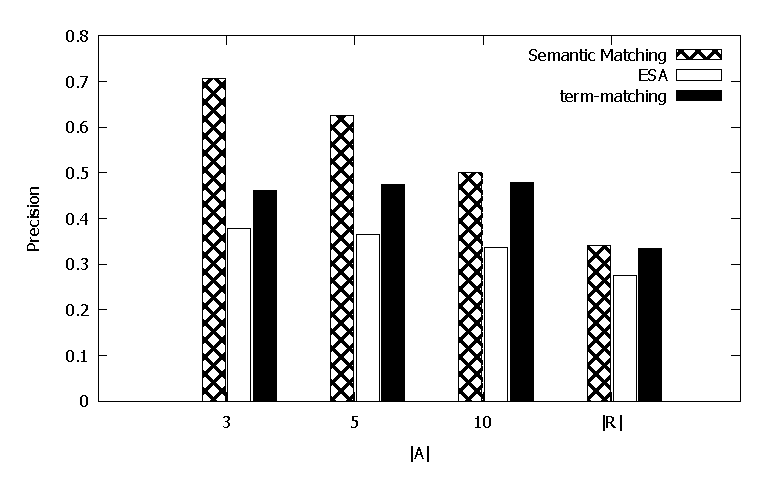
\epsfig{file=figures/precision.eps,height=1.2in,width=2.2in}
            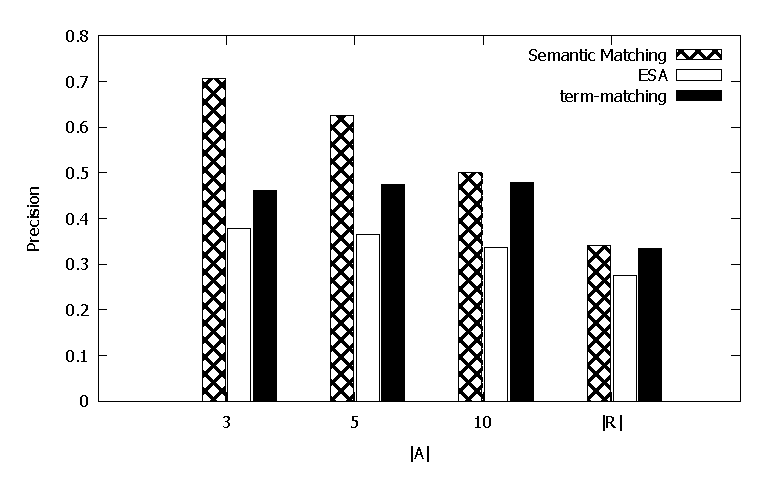
\includegraphics[height=1.2in,
                width=2.2in]{figures/precision.eps}
        \end{minipage}
    }
    \subfigure[Compare Nonobvious]{
        \label{fig:subfig:b2}
        \begin{minipage}[b]{0.33\textwidth}
            \centering
            %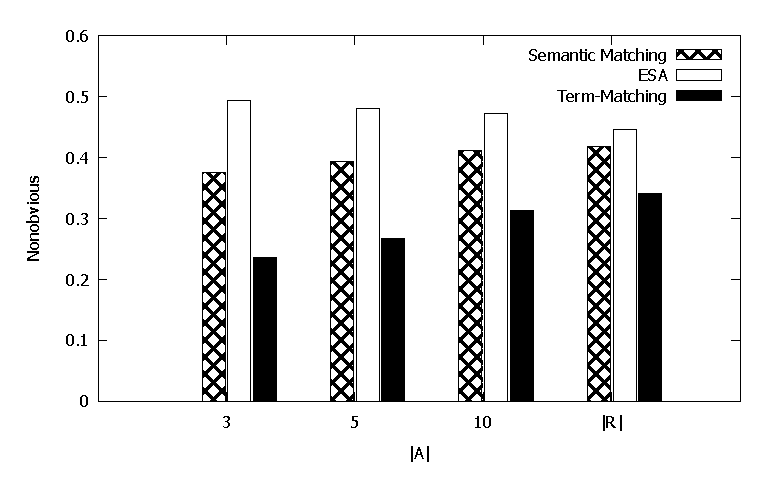
\epsfig{file=figures/nonobvious.eps,height=1.2in,width=2.2in}
            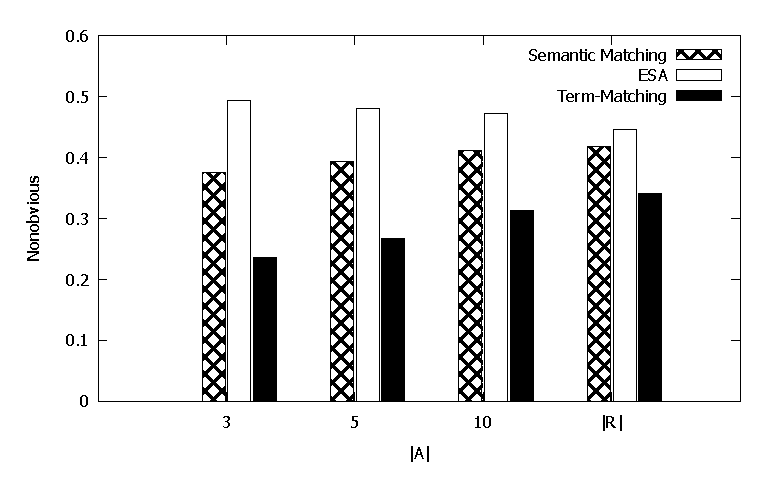
\includegraphics[height=1.2in,
                width=2.2in]{figures/nonobvious.eps}
        \end{minipage}
    }
    \subfigure[Compare Precision+Nonobvious]{
        \label{fig:subfig:c2}
        \begin{minipage}[b]{0.33\textwidth}
            \centering
            %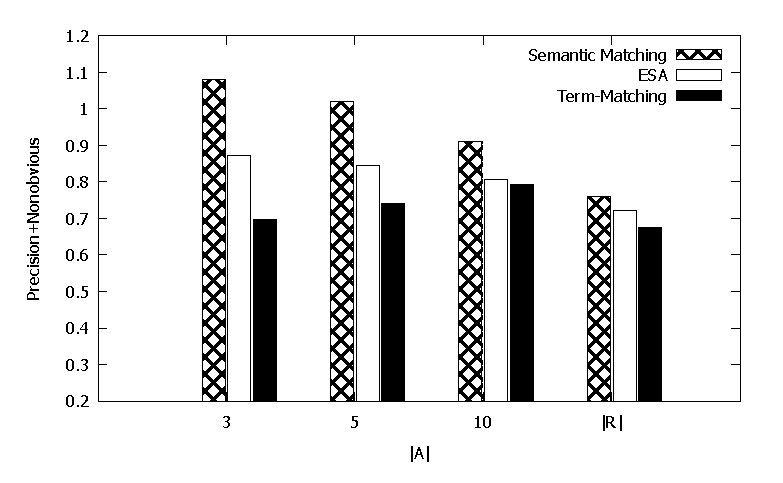
\epsfig{file=figures/plus.eps,height=1.2in,width=2.2in}
            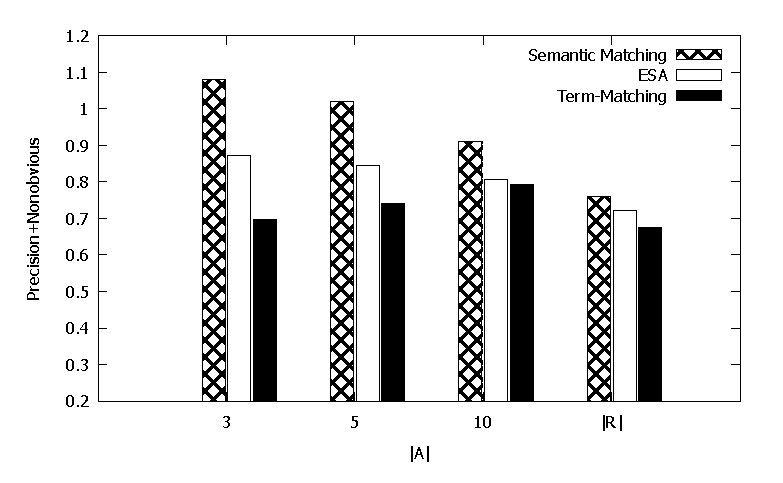
\includegraphics[width=2.2in,
                height=1.2in]{figures/plus.eps}
        \end{minipage}
    }
\caption{Evaluation using Keyword Research Service}
\label{fig:expadcenter}
\end{figure*}
Our semantic matching approach outperform ESA and term-vector
approach on the metrics \emph{p@n} which comfirms the
effectiveness of our approach from the perspective of information
retrieval.
Because both ESA and our approach model short text at semantic
level while standard bag of words technique simply characterizes each
short text as set of terms, the metrics \emph{nonobvious score} is intrinsically
inclined to ESA and our approach.



%\subsubsection{Massive Dataset and User Study}
\subsection{Performance over Massive Dataset}
\textbf{Objective} of this experiment is mainly to confirm the
scalability of our approach.
Besides, since bid phrases provided by keyword search tool is selected
by algorithms instead of human beings, We held user study to assess
the relevance between queries and retrieved bid phrases.



\textbf{Dataset} for our evaluation purpose includes a set of testing
queries and a extremely huge corpus of bid phrases.
For the convenience of user study, we select 50 queries from our query
set that are easy for participators to interpret.
Because previous experiment compare our approach with several
baselines over a corpus of ordinary size(300k bid phrases), we
adopt the whole keyword set for this experiment.



\textbf{Metrics} of this experiment is p@n.
Because our human resource is limited, we give up graded relevance
assessments such as NDCG and thus choose p@n which allow only binary
assessments.
For each test query, we apply different approaches to selecting bid
phrases from our massive corpus respectively.
Then participators are asked to label each result as relevant or not
according to their own subjective judgment.
There are totally five participators and all of them are experienced
web users.



%For each of these sampled queries, we select top-$10$ bid phrases by our
%approach from a huge corpus consisting of 0.702 billion bid phrases
%provided by a commercial search engine.
%We adopt such a extremely huge corpus to confirm that our approach has
%the scalability to be applied for such massive dataset.
%These queries' most relevant expansions are also extracted to be used
%as baseline\comment{what?}.
\textbf{Baseline} of this experiment is not certain keyword suggestion
or query expansion approach.
%, but the most successful bid phrases with
%respect to our test queries provided by a commercial search engine.
Instead, we use each test query's expansions provided by commercial
search engine as baseline.
The expansions of queries are bid phrases which have the highest
\emph{CTR}.
%Participators are asked to score each resulting bid phrase according to labeling guidline listed in Table
%\ref{tab:scoringrule} without the information that bid
%phrases are generated by a certain approach.

%Since our corpus consists of totally 0.702 billion bid phrases, it's impossible
%for human beings to count the exact number of relevant ones with
%respect to a given query within the corpus.
%Thus, we compared the quality of expansions generated by our
%approach and those provided by search engine using \emph{p@n} as
%metrics.
%Because we asked users to label results in a stage manner(i.e., we do
%        not label bid phrases as black or white but assign a score to
%        each one), we define \emph{p@n} slightly different from
%conventional one.
%Actually, we define it to be the summation of labeled scores of top-$n$
%bid phrases divided by $3\times n$.
%We consider cases where $n=1, 3, 5, 10$.
%The comparison is illustrated in the Table \ref{tab:vsbing}.
For some test queries, the number of relevant bid phrases provided by
the search engine is less than 10, so we have to present the
\emph{p@10} only of our approach.



\textbf{Experiment results} are illustrated in Table \ref{tab:vsbing}.
For small $n$, our approach achieve obvious
improvement compared with the commercial search engine.
Because the number of ads displayed for one search is much less
than the number of web pages returned to search users, the relevance
between top ranked bid phrases and given query is critical.
Therefore, the advantage of our approach is significant.
%We have claimed that our approach is suitable for applying to massive
%dataset, so we evaluate our approach using 702 millions of bid
%keywords indexed by Bing search engine.
%We randomly sampled 42 quries including head queries as well as torso
%and tail queries, from search log and generate top 5 most related bid
%keywords for each query as resulting expansion by our approach.
%We also extracted the expansion results for these queries generated by
%Bing search engine.
%For comparison purpose, we held user study where each participator is
%asked to score each resulting bid keyword according to pre-defined
%rule.
%Table \ref{tab:scoringrule} presents scoring rule adopted in our user study.
%We labeled resulting bid keywords in a stage manner expecting to give
%them more precise description and present the relationship between
%queries and bid keywords rather than simply judging them as relevant
%or not.
%\begin{table}
%\centering
%\caption{Scoring Rule}
%\begin{tabular}{|c|c|c|c|} \hline
%Score&Relationship&Query&Bid Keyword\\ \hline
%3&same&car insurance&automatic insurance\\ \hline
%2&specific&car rental&car rental LA\\ \hline
%2&general&iphone&apple product\\ \hline
%2&overlap&fruit ninja xbox&fruit ninja for ios\\ \hline
%1&disjoint&hot dog&dog\\ \hline
%\end{tabular}
%\label{tab:scoringrule}
%\end{table}
%Since the total corpus contains about 702 millions of bid keywords, we
%have no idea about the exact number of related bid keywords for a given
%query which is required for computing precision and recall.
%We compared the performance of our approach with Bing search engine by
%comparing \emph{p@n} which is also a conventional metrics for evaluating
%informaion retrieval systems.
%Here we consider cases where $n=1, 3, 5$.
%As we know, \emph{p@n} is computed by dividing the number of positive
%ones in the top-$n$ by $n$ where testing data is labeled in a black or
%white manner.
%So we have to make some modification to \emph{p@n} for our cases.
%Here we define it to be the summation of scores of top-$n$ bid
%keywords divided by $3\times n$.
%The comparison is illustrated in the Table 3.
\begin{table}
\centering
\begin{tabular}{|c|c|c|} \hline
$p@n$&Search Engine&Our Approach\\ \hline
$n=1$&$0.778$&$0.827$\\ \hline
$n=3$&$0.729$&$0.784$\\ \hline
$n=5$&$0.723$&$0.755$\\ \hline
$n=10$&&$0.717$\\ \hline
\end{tabular}
\caption{Comparison between Our Approach and Bing Search Engine}
\label{tab:vsbing}
\end{table}
%\subsection{Pruning}
%In reality, search engine preprocesses a list of queries offline and
%builds inverted index for the resulting expansions(query as term and
%    its expansion as corresponding posting list).
%At runtime, search engine uses the resulting expansions to find
%relevant bid keywords for submitted query.
%When there is enough traffic volumne to ensure computed metrics(e.g.,
%        click through rate(CTR), cost per click(CPC), etc.) reliable,
%     search engine will analyze and prune those bad expansion.
%For example, a certain bid keyword is high-ranking in the expansion
%for a certain query.
%However, the CTR for ads retrieved through this bid keyword is so low.
%This bid keyword may be not so relevant to that query and search
%engine will eliminate it from that query's expansion in the next
%version.
%Although pruning is not an elegant approach to improve effectiveness
%of sponsored search, it is an important and indespensable step of
%sponsored search adopted by many mainstream search engines.
%
%
%Different from latent semantic analysis approaches which represent
%documents as distribution over latent topics and topics as
%distributions over vocabulary of indexed corpus, our approach
%represents documents as explicit topics where topics are concepts used
%in our daily life.
%Such a representation of the meaning behind any text is
%easy to explain to human users\cite{gabrilovich:semanticanalysis}.
%By our explicit representation of semantic meaning, we are able to not
%only prune resulting expansion based on conventioinal metrics but also
%infer and analyze more detailed problem behind the symptom such as
%which topics(concepts) contain commercial intent, which domains our
%approach can't not generate useful expansions.
%For example, when we find that CTRs of expansions for queries related
%to concept ``hotel'' are lower than other topics(concepts),
%we can collect these queries and design vertical search engine for
%this specific domain.

\section{Conclusion}
In this paper, we proposed a novel approach for keyword suggestion and
query expansion.
We also conducted a series of experiments to evaluate our approach and 
%It can also be applied to general text modeling tasks over corpus of
%short text snippets without any modification.
the experiment results show that our approach can successfully select
relevant yet not so obvious bid phrases for a given query no matter
the query is popular or rare.
Since most existing approaches exploiting historical data can't be
applied to tail queries, this fact confirms that directly making use
of semantic knowledge is helpful for sponsored search.
%reveal that modeling a corpus of shot text
%snippets with the help of rich common sense knowledge is an effective
%way.
Besides, our approach outperforms ESA that also model
text snippets as explicit concepts, which gives approval to both
Probase and conceptualization algorithm proposed in this paper.
%However, our conceptualization approach is highlighted by WSD phase
%which leverages large scale co-occurrence network not so elegantly.
%We will continue to seek conceptualization approach that absorbs the WSD phrase
%into our inferrence phase and functions in an purely probabilistic
%way.


% The following two commands are all you need in the
% initial runs of your .tex file to
% produce the bibliography for the citations in your paper.
\bibliographystyle{abbrv}
\bibliography{adselection}  % sigproc.bib is the name of the Bibliography in this case
% You must have a proper ".bib" file
%  and remember to run:
% latex bibtex latex latex
% to resolve all references
\end{document}


